\documentclass[twoside]{book}

% Packages required by doxygen
\usepackage{fixltx2e}
\usepackage{calc}
\usepackage{doxygen}
\usepackage[export]{adjustbox} % also loads graphicx
\usepackage{graphicx}
\usepackage[utf8]{inputenc}
\usepackage{makeidx}
\usepackage{multicol}
\usepackage{multirow}
\PassOptionsToPackage{warn}{textcomp}
\usepackage{textcomp}
\usepackage[nointegrals]{wasysym}
\usepackage[table]{xcolor}

% Font selection
\usepackage[T1]{fontenc}
\usepackage[scaled=.90]{helvet}
\usepackage{courier}
\usepackage{amssymb}
\usepackage{sectsty}
\renewcommand{\familydefault}{\sfdefault}
\allsectionsfont{%
  \fontseries{bc}\selectfont%
  \color{darkgray}%
}
\renewcommand{\DoxyLabelFont}{%
  \fontseries{bc}\selectfont%
  \color{darkgray}%
}
\newcommand{\+}{\discretionary{\mbox{\scriptsize$\hookleftarrow$}}{}{}}

% Page & text layout
\usepackage{geometry}
\geometry{%
  a4paper,%
  top=2.5cm,%
  bottom=2.5cm,%
  left=2.5cm,%
  right=2.5cm%
}
\tolerance=750
\hfuzz=15pt
\hbadness=750
\setlength{\emergencystretch}{15pt}
\setlength{\parindent}{0cm}
\setlength{\parskip}{3ex plus 2ex minus 2ex}
\makeatletter
\renewcommand{\paragraph}{%
  \@startsection{paragraph}{4}{0ex}{-1.0ex}{1.0ex}{%
    \normalfont\normalsize\bfseries\SS@parafont%
  }%
}
\renewcommand{\subparagraph}{%
  \@startsection{subparagraph}{5}{0ex}{-1.0ex}{1.0ex}{%
    \normalfont\normalsize\bfseries\SS@subparafont%
  }%
}
\makeatother

% Headers & footers
\usepackage{fancyhdr}
\pagestyle{fancyplain}
\fancyhead[LE]{\fancyplain{}{\bfseries\thepage}}
\fancyhead[CE]{\fancyplain{}{}}
\fancyhead[RE]{\fancyplain{}{\bfseries\leftmark}}
\fancyhead[LO]{\fancyplain{}{\bfseries\rightmark}}
\fancyhead[CO]{\fancyplain{}{}}
\fancyhead[RO]{\fancyplain{}{\bfseries\thepage}}
\fancyfoot[LE]{\fancyplain{}{}}
\fancyfoot[CE]{\fancyplain{}{}}
\fancyfoot[RE]{\fancyplain{}{\bfseries\scriptsize Generated by Doxygen }}
\fancyfoot[LO]{\fancyplain{}{\bfseries\scriptsize Generated by Doxygen }}
\fancyfoot[CO]{\fancyplain{}{}}
\fancyfoot[RO]{\fancyplain{}{}}
\renewcommand{\footrulewidth}{0.4pt}
\renewcommand{\chaptermark}[1]{%
  \markboth{#1}{}%
}
\renewcommand{\sectionmark}[1]{%
  \markright{\thesection\ #1}%
}

% Indices & bibliography
\usepackage{natbib}
\usepackage[titles]{tocloft}
\setcounter{tocdepth}{3}
\setcounter{secnumdepth}{5}
\makeindex

% Hyperlinks (required, but should be loaded last)
\usepackage{ifpdf}
\ifpdf
  \usepackage[pdftex,pagebackref=true]{hyperref}
\else
  \usepackage[ps2pdf,pagebackref=true]{hyperref}
\fi
\hypersetup{%
  colorlinks=true,%
  linkcolor=blue,%
  citecolor=blue,%
  unicode%
}

% Custom commands
\newcommand{\clearemptydoublepage}{%
  \newpage{\pagestyle{empty}\cleardoublepage}%
}

\usepackage{caption}
\captionsetup{labelsep=space,justification=centering,font={bf},singlelinecheck=off,skip=4pt,position=top}

%===== C O N T E N T S =====

\begin{document}

% Titlepage & ToC
\hypersetup{pageanchor=false,
             bookmarksnumbered=true,
             pdfencoding=unicode
            }
\pagenumbering{alph}
\begin{titlepage}
\vspace*{7cm}
\begin{center}%
{\Large cxx\+\_\+chebyshev }\\
\vspace*{1cm}
{\large Generated by Doxygen 1.8.13}\\
\end{center}
\end{titlepage}
\clearemptydoublepage
\pagenumbering{roman}
\tableofcontents
\clearemptydoublepage
\pagenumbering{arabic}
\hypersetup{pageanchor=true}

%--- Begin generated contents ---
\chapter{Namespace Index}
\section{Namespace List}
Here is a list of all namespaces with brief descriptions\+:\begin{DoxyCompactList}
\item\contentsline{section}{\hyperlink{namespace____gnu__cxx}{\+\_\+\+\_\+gnu\+\_\+cxx} }{\pageref{namespace____gnu__cxx}}{}
\item\contentsline{section}{\hyperlink{namespace____gnu__cxx_1_1detail}{\+\_\+\+\_\+gnu\+\_\+cxx\+::detail} }{\pageref{namespace____gnu__cxx_1_1detail}}{}
\end{DoxyCompactList}

\chapter{Class Index}
\section{Class List}
Here are the classes, structs, unions and interfaces with brief descriptions\+:\begin{DoxyCompactList}
\item\contentsline{section}{\hyperlink{struct____gnu__cxx_1_1____airy__t}{\+\_\+\+\_\+gnu\+\_\+cxx\+::\+\_\+\+\_\+airy\+\_\+t$<$ \+\_\+\+Tx, \+\_\+\+Tp $>$} }{\pageref{struct____gnu__cxx_1_1____airy__t}}{}
\item\contentsline{section}{\hyperlink{struct____gnu__cxx_1_1____cyl__bessel__t}{\+\_\+\+\_\+gnu\+\_\+cxx\+::\+\_\+\+\_\+cyl\+\_\+bessel\+\_\+t$<$ \+\_\+\+Tnu, \+\_\+\+Tx, \+\_\+\+Tp $>$} }{\pageref{struct____gnu__cxx_1_1____cyl__bessel__t}}{}
\item\contentsline{section}{\hyperlink{struct____gnu__cxx_1_1____cyl__hankel__t}{\+\_\+\+\_\+gnu\+\_\+cxx\+::\+\_\+\+\_\+cyl\+\_\+hankel\+\_\+t$<$ \+\_\+\+Tnu, \+\_\+\+Tx, \+\_\+\+Tp $>$} }{\pageref{struct____gnu__cxx_1_1____cyl__hankel__t}}{}
\item\contentsline{section}{\hyperlink{struct____gnu__cxx_1_1____cyl__mod__bessel__t}{\+\_\+\+\_\+gnu\+\_\+cxx\+::\+\_\+\+\_\+cyl\+\_\+mod\+\_\+bessel\+\_\+t$<$ \+\_\+\+Tnu, \+\_\+\+Tx, \+\_\+\+Tp $>$} }{\pageref{struct____gnu__cxx_1_1____cyl__mod__bessel__t}}{}
\item\contentsline{section}{\hyperlink{struct____gnu__cxx_1_1____fock__airy__t}{\+\_\+\+\_\+gnu\+\_\+cxx\+::\+\_\+\+\_\+fock\+\_\+airy\+\_\+t$<$ \+\_\+\+Tx, \+\_\+\+Tp $>$} }{\pageref{struct____gnu__cxx_1_1____fock__airy__t}}{}
\item\contentsline{section}{\hyperlink{struct____gnu__cxx_1_1____fp__is__integer__t}{\+\_\+\+\_\+gnu\+\_\+cxx\+::\+\_\+\+\_\+fp\+\_\+is\+\_\+integer\+\_\+t} }{\pageref{struct____gnu__cxx_1_1____fp__is__integer__t}}{}
\item\contentsline{section}{\hyperlink{struct____gnu__cxx_1_1____gamma__inc__t}{\+\_\+\+\_\+gnu\+\_\+cxx\+::\+\_\+\+\_\+gamma\+\_\+inc\+\_\+t$<$ \+\_\+\+Tp $>$} }{\pageref{struct____gnu__cxx_1_1____gamma__inc__t}}{}
\item\contentsline{section}{\hyperlink{struct____gnu__cxx_1_1____gamma__temme__t}{\+\_\+\+\_\+gnu\+\_\+cxx\+::\+\_\+\+\_\+gamma\+\_\+temme\+\_\+t$<$ \+\_\+\+Tp $>$} \\*A structure for the gamma functions required by the Temme series expansions of $ N_\nu(x) $ and $ K_\nu(x) $. \[ \Gamma_1 = \frac{1}{2\mu} \left[\frac{1}{\Gamma(1 - \mu)} - \frac{1}{\Gamma(1 + \mu)}\right] \] and \[ \Gamma_2 = \frac{1}{2} \left[\frac{1}{\Gamma(1 - \mu)} + \frac{1}{\Gamma(1 + \mu)}\right] \] where $ -1/2 <= \mu <= 1/2 $ is $ \mu = \nu - N $ and $ N $. is the nearest integer to $ \nu $. The values of $ \Gamma(1 + \mu) $ and $ \Gamma(1 - \mu) $ are returned as well }{\pageref{struct____gnu__cxx_1_1____gamma__temme__t}}{}
\item\contentsline{section}{\hyperlink{struct____gnu__cxx_1_1____jacobi__t}{\+\_\+\+\_\+gnu\+\_\+cxx\+::\+\_\+\+\_\+jacobi\+\_\+t$<$ \+\_\+\+Tp $>$} }{\pageref{struct____gnu__cxx_1_1____jacobi__t}}{}
\item\contentsline{section}{\hyperlink{struct____gnu__cxx_1_1____lgamma__t}{\+\_\+\+\_\+gnu\+\_\+cxx\+::\+\_\+\+\_\+lgamma\+\_\+t$<$ \+\_\+\+Tp $>$} }{\pageref{struct____gnu__cxx_1_1____lgamma__t}}{}
\item\contentsline{section}{\hyperlink{struct____gnu__cxx_1_1____pqgamma__t}{\+\_\+\+\_\+gnu\+\_\+cxx\+::\+\_\+\+\_\+pqgamma\+\_\+t$<$ \+\_\+\+Tp $>$} }{\pageref{struct____gnu__cxx_1_1____pqgamma__t}}{}
\item\contentsline{section}{\hyperlink{struct____gnu__cxx_1_1____quadrature__point__t}{\+\_\+\+\_\+gnu\+\_\+cxx\+::\+\_\+\+\_\+quadrature\+\_\+point\+\_\+t$<$ \+\_\+\+Tp $>$} }{\pageref{struct____gnu__cxx_1_1____quadrature__point__t}}{}
\item\contentsline{section}{\hyperlink{struct____gnu__cxx_1_1____sincos__t}{\+\_\+\+\_\+gnu\+\_\+cxx\+::\+\_\+\+\_\+sincos\+\_\+t$<$ \+\_\+\+Tp $>$} }{\pageref{struct____gnu__cxx_1_1____sincos__t}}{}
\item\contentsline{section}{\hyperlink{struct____gnu__cxx_1_1____sph__bessel__t}{\+\_\+\+\_\+gnu\+\_\+cxx\+::\+\_\+\+\_\+sph\+\_\+bessel\+\_\+t$<$ \+\_\+\+Tn, \+\_\+\+Tx, \+\_\+\+Tp $>$} }{\pageref{struct____gnu__cxx_1_1____sph__bessel__t}}{}
\item\contentsline{section}{\hyperlink{struct____gnu__cxx_1_1____sph__hankel__t}{\+\_\+\+\_\+gnu\+\_\+cxx\+::\+\_\+\+\_\+sph\+\_\+hankel\+\_\+t$<$ \+\_\+\+Tn, \+\_\+\+Tx, \+\_\+\+Tp $>$} }{\pageref{struct____gnu__cxx_1_1____sph__hankel__t}}{}
\item\contentsline{section}{\hyperlink{struct____gnu__cxx_1_1____sph__mod__bessel__t}{\+\_\+\+\_\+gnu\+\_\+cxx\+::\+\_\+\+\_\+sph\+\_\+mod\+\_\+bessel\+\_\+t$<$ \+\_\+\+Tn, \+\_\+\+Tx, \+\_\+\+Tp $>$} }{\pageref{struct____gnu__cxx_1_1____sph__mod__bessel__t}}{}
\item\contentsline{section}{\hyperlink{structstd_1_1____detail_1_1____gamma__lanczos__data}{std\+::\+\_\+\+\_\+detail\+::\+\_\+\+\_\+gamma\+\_\+lanczos\+\_\+data$<$ \+\_\+\+Tp $>$} }{\pageref{structstd_1_1____detail_1_1____gamma__lanczos__data}}{}
\item\contentsline{section}{\hyperlink{structstd_1_1____detail_1_1____gamma__lanczos__data_3_01double_01_4}{std\+::\+\_\+\+\_\+detail\+::\+\_\+\+\_\+gamma\+\_\+lanczos\+\_\+data$<$ double $>$} }{\pageref{structstd_1_1____detail_1_1____gamma__lanczos__data_3_01double_01_4}}{}
\item\contentsline{section}{\hyperlink{structstd_1_1____detail_1_1____gamma__lanczos__data_3_01float_01_4}{std\+::\+\_\+\+\_\+detail\+::\+\_\+\+\_\+gamma\+\_\+lanczos\+\_\+data$<$ float $>$} }{\pageref{structstd_1_1____detail_1_1____gamma__lanczos__data_3_01float_01_4}}{}
\item\contentsline{section}{\hyperlink{structstd_1_1____detail_1_1____gamma__lanczos__data_3_01long_01double_01_4}{std\+::\+\_\+\+\_\+detail\+::\+\_\+\+\_\+gamma\+\_\+lanczos\+\_\+data$<$ long double $>$} }{\pageref{structstd_1_1____detail_1_1____gamma__lanczos__data_3_01long_01double_01_4}}{}
\item\contentsline{section}{\hyperlink{structstd_1_1____detail_1_1____gamma__spouge__data}{std\+::\+\_\+\+\_\+detail\+::\+\_\+\+\_\+gamma\+\_\+spouge\+\_\+data$<$ \+\_\+\+Tp $>$} }{\pageref{structstd_1_1____detail_1_1____gamma__spouge__data}}{}
\item\contentsline{section}{\hyperlink{structstd_1_1____detail_1_1____gamma__spouge__data_3_01double_01_4}{std\+::\+\_\+\+\_\+detail\+::\+\_\+\+\_\+gamma\+\_\+spouge\+\_\+data$<$ double $>$} }{\pageref{structstd_1_1____detail_1_1____gamma__spouge__data_3_01double_01_4}}{}
\item\contentsline{section}{\hyperlink{structstd_1_1____detail_1_1____gamma__spouge__data_3_01float_01_4}{std\+::\+\_\+\+\_\+detail\+::\+\_\+\+\_\+gamma\+\_\+spouge\+\_\+data$<$ float $>$} }{\pageref{structstd_1_1____detail_1_1____gamma__spouge__data_3_01float_01_4}}{}
\item\contentsline{section}{\hyperlink{structstd_1_1____detail_1_1____gamma__spouge__data_3_01long_01double_01_4}{std\+::\+\_\+\+\_\+detail\+::\+\_\+\+\_\+gamma\+\_\+spouge\+\_\+data$<$ long double $>$} }{\pageref{structstd_1_1____detail_1_1____gamma__spouge__data_3_01long_01double_01_4}}{}
\item\contentsline{section}{\hyperlink{classstd_1_1____detail_1_1__Airy}{std\+::\+\_\+\+\_\+detail\+::\+\_\+\+Airy$<$ \+\_\+\+Tp $>$} }{\pageref{classstd_1_1____detail_1_1__Airy}}{}
\item\contentsline{section}{\hyperlink{classstd_1_1____detail_1_1__Airy__asymp}{std\+::\+\_\+\+\_\+detail\+::\+\_\+\+Airy\+\_\+asymp$<$ \+\_\+\+Tp $>$} }{\pageref{classstd_1_1____detail_1_1__Airy__asymp}}{}
\item\contentsline{section}{\hyperlink{structstd_1_1____detail_1_1__Airy__asymp__data}{std\+::\+\_\+\+\_\+detail\+::\+\_\+\+Airy\+\_\+asymp\+\_\+data$<$ \+\_\+\+Tp $>$} }{\pageref{structstd_1_1____detail_1_1__Airy__asymp__data}}{}
\item\contentsline{section}{\hyperlink{structstd_1_1____detail_1_1__Airy__asymp__data_3_01double_01_4}{std\+::\+\_\+\+\_\+detail\+::\+\_\+\+Airy\+\_\+asymp\+\_\+data$<$ double $>$} }{\pageref{structstd_1_1____detail_1_1__Airy__asymp__data_3_01double_01_4}}{}
\item\contentsline{section}{\hyperlink{structstd_1_1____detail_1_1__Airy__asymp__data_3_01float_01_4}{std\+::\+\_\+\+\_\+detail\+::\+\_\+\+Airy\+\_\+asymp\+\_\+data$<$ float $>$} }{\pageref{structstd_1_1____detail_1_1__Airy__asymp__data_3_01float_01_4}}{}
\item\contentsline{section}{\hyperlink{structstd_1_1____detail_1_1__Airy__asymp__data_3_01long_01double_01_4}{std\+::\+\_\+\+\_\+detail\+::\+\_\+\+Airy\+\_\+asymp\+\_\+data$<$ long double $>$} }{\pageref{structstd_1_1____detail_1_1__Airy__asymp__data_3_01long_01double_01_4}}{}
\item\contentsline{section}{\hyperlink{classstd_1_1____detail_1_1__Airy__asymp__series}{std\+::\+\_\+\+\_\+detail\+::\+\_\+\+Airy\+\_\+asymp\+\_\+series$<$ \+\_\+\+Sum $>$} }{\pageref{classstd_1_1____detail_1_1__Airy__asymp__series}}{}
\item\contentsline{section}{\hyperlink{structstd_1_1____detail_1_1__Airy__default__radii}{std\+::\+\_\+\+\_\+detail\+::\+\_\+\+Airy\+\_\+default\+\_\+radii$<$ \+\_\+\+Tp $>$} }{\pageref{structstd_1_1____detail_1_1__Airy__default__radii}}{}
\item\contentsline{section}{\hyperlink{structstd_1_1____detail_1_1__Airy__default__radii_3_01double_01_4}{std\+::\+\_\+\+\_\+detail\+::\+\_\+\+Airy\+\_\+default\+\_\+radii$<$ double $>$} }{\pageref{structstd_1_1____detail_1_1__Airy__default__radii_3_01double_01_4}}{}
\item\contentsline{section}{\hyperlink{structstd_1_1____detail_1_1__Airy__default__radii_3_01float_01_4}{std\+::\+\_\+\+\_\+detail\+::\+\_\+\+Airy\+\_\+default\+\_\+radii$<$ float $>$} }{\pageref{structstd_1_1____detail_1_1__Airy__default__radii_3_01float_01_4}}{}
\item\contentsline{section}{\hyperlink{structstd_1_1____detail_1_1__Airy__default__radii_3_01long_01double_01_4}{std\+::\+\_\+\+\_\+detail\+::\+\_\+\+Airy\+\_\+default\+\_\+radii$<$ long double $>$} }{\pageref{structstd_1_1____detail_1_1__Airy__default__radii_3_01long_01double_01_4}}{}
\item\contentsline{section}{\hyperlink{classstd_1_1____detail_1_1__Airy__series}{std\+::\+\_\+\+\_\+detail\+::\+\_\+\+Airy\+\_\+series$<$ \+\_\+\+Tp $>$} }{\pageref{classstd_1_1____detail_1_1__Airy__series}}{}
\item\contentsline{section}{\hyperlink{structstd_1_1____detail_1_1__AiryAuxilliaryState}{std\+::\+\_\+\+\_\+detail\+::\+\_\+\+Airy\+Auxilliary\+State$<$ \+\_\+\+Tp $>$} }{\pageref{structstd_1_1____detail_1_1__AiryAuxilliaryState}}{}
\item\contentsline{section}{\hyperlink{structstd_1_1____detail_1_1__AiryState}{std\+::\+\_\+\+\_\+detail\+::\+\_\+\+Airy\+State$<$ \+\_\+\+Tp $>$} }{\pageref{structstd_1_1____detail_1_1__AiryState}}{}
\item\contentsline{section}{\hyperlink{structstd_1_1____detail_1_1__Factorial__table}{std\+::\+\_\+\+\_\+detail\+::\+\_\+\+Factorial\+\_\+table$<$ \+\_\+\+Tp $>$} }{\pageref{structstd_1_1____detail_1_1__Factorial__table}}{}
\end{DoxyCompactList}

\chapter{File Index}
\section{File List}
Here is a list of all files with brief descriptions\+:\begin{DoxyCompactList}
\item\contentsline{section}{bits/\hyperlink{sf__airy_8tcc}{sf\+\_\+airy.\+tcc} }{\pageref{sf__airy_8tcc}}{}
\item\contentsline{section}{bits/\hyperlink{sf__bernoulli_8tcc}{sf\+\_\+bernoulli.\+tcc} }{\pageref{sf__bernoulli_8tcc}}{}
\item\contentsline{section}{bits/\hyperlink{sf__bessel_8tcc}{sf\+\_\+bessel.\+tcc} }{\pageref{sf__bessel_8tcc}}{}
\item\contentsline{section}{bits/\hyperlink{sf__beta_8tcc}{sf\+\_\+beta.\+tcc} }{\pageref{sf__beta_8tcc}}{}
\item\contentsline{section}{bits/\hyperlink{sf__cardinal_8tcc}{sf\+\_\+cardinal.\+tcc} }{\pageref{sf__cardinal_8tcc}}{}
\item\contentsline{section}{bits/\hyperlink{sf__chebyshev_8tcc}{sf\+\_\+chebyshev.\+tcc} }{\pageref{sf__chebyshev_8tcc}}{}
\item\contentsline{section}{bits/\hyperlink{sf__coulomb_8tcc}{sf\+\_\+coulomb.\+tcc} }{\pageref{sf__coulomb_8tcc}}{}
\item\contentsline{section}{bits/\hyperlink{sf__dawson_8tcc}{sf\+\_\+dawson.\+tcc} }{\pageref{sf__dawson_8tcc}}{}
\item\contentsline{section}{bits/\hyperlink{sf__distributions_8tcc}{sf\+\_\+distributions.\+tcc} }{\pageref{sf__distributions_8tcc}}{}
\item\contentsline{section}{bits/\hyperlink{sf__ellint_8tcc}{sf\+\_\+ellint.\+tcc} }{\pageref{sf__ellint_8tcc}}{}
\item\contentsline{section}{bits/\hyperlink{sf__euler_8tcc}{sf\+\_\+euler.\+tcc} }{\pageref{sf__euler_8tcc}}{}
\item\contentsline{section}{bits/\hyperlink{sf__expint_8tcc}{sf\+\_\+expint.\+tcc} }{\pageref{sf__expint_8tcc}}{}
\item\contentsline{section}{bits/\hyperlink{sf__fresnel_8tcc}{sf\+\_\+fresnel.\+tcc} }{\pageref{sf__fresnel_8tcc}}{}
\item\contentsline{section}{bits/\hyperlink{sf__gamma_8tcc}{sf\+\_\+gamma.\+tcc} }{\pageref{sf__gamma_8tcc}}{}
\item\contentsline{section}{bits/\hyperlink{sf__gegenbauer_8tcc}{sf\+\_\+gegenbauer.\+tcc} }{\pageref{sf__gegenbauer_8tcc}}{}
\item\contentsline{section}{bits/\hyperlink{sf__hankel_8tcc}{sf\+\_\+hankel.\+tcc} }{\pageref{sf__hankel_8tcc}}{}
\item\contentsline{section}{bits/\hyperlink{sf__hermite_8tcc}{sf\+\_\+hermite.\+tcc} }{\pageref{sf__hermite_8tcc}}{}
\item\contentsline{section}{bits/\hyperlink{sf__hyperg_8tcc}{sf\+\_\+hyperg.\+tcc} }{\pageref{sf__hyperg_8tcc}}{}
\item\contentsline{section}{bits/\hyperlink{sf__hypint_8tcc}{sf\+\_\+hypint.\+tcc} }{\pageref{sf__hypint_8tcc}}{}
\item\contentsline{section}{bits/\hyperlink{sf__jacobi_8tcc}{sf\+\_\+jacobi.\+tcc} }{\pageref{sf__jacobi_8tcc}}{}
\item\contentsline{section}{bits/\hyperlink{sf__laguerre_8tcc}{sf\+\_\+laguerre.\+tcc} }{\pageref{sf__laguerre_8tcc}}{}
\item\contentsline{section}{bits/\hyperlink{sf__legendre_8tcc}{sf\+\_\+legendre.\+tcc} }{\pageref{sf__legendre_8tcc}}{}
\item\contentsline{section}{bits/\hyperlink{sf__mod__bessel_8tcc}{sf\+\_\+mod\+\_\+bessel.\+tcc} }{\pageref{sf__mod__bessel_8tcc}}{}
\item\contentsline{section}{bits/\hyperlink{sf__owens__t_8tcc}{sf\+\_\+owens\+\_\+t.\+tcc} }{\pageref{sf__owens__t_8tcc}}{}
\item\contentsline{section}{bits/\hyperlink{sf__polylog_8tcc}{sf\+\_\+polylog.\+tcc} }{\pageref{sf__polylog_8tcc}}{}
\item\contentsline{section}{bits/\hyperlink{sf__stirling_8tcc}{sf\+\_\+stirling.\+tcc} }{\pageref{sf__stirling_8tcc}}{}
\item\contentsline{section}{bits/\hyperlink{sf__theta_8tcc}{sf\+\_\+theta.\+tcc} }{\pageref{sf__theta_8tcc}}{}
\item\contentsline{section}{bits/\hyperlink{sf__trig_8tcc}{sf\+\_\+trig.\+tcc} }{\pageref{sf__trig_8tcc}}{}
\item\contentsline{section}{bits/\hyperlink{sf__trigint_8tcc}{sf\+\_\+trigint.\+tcc} }{\pageref{sf__trigint_8tcc}}{}
\item\contentsline{section}{bits/\hyperlink{sf__zeta_8tcc}{sf\+\_\+zeta.\+tcc} }{\pageref{sf__zeta_8tcc}}{}
\item\contentsline{section}{bits/\hyperlink{specfun_8h}{specfun.\+h} }{\pageref{specfun_8h}}{}
\item\contentsline{section}{bits/\hyperlink{specfun__state_8h}{specfun\+\_\+state.\+h} }{\pageref{specfun__state_8h}}{}
\item\contentsline{section}{ext/\hyperlink{math__util_8h}{math\+\_\+util.\+h} }{\pageref{math__util_8h}}{}
\end{DoxyCompactList}

\chapter{Namespace Documentation}
\hypertarget{namespace____gnu__cxx}{}\section{\+\_\+\+\_\+gnu\+\_\+cxx Namespace Reference}
\label{namespace____gnu__cxx}\index{\+\_\+\+\_\+gnu\+\_\+cxx@{\+\_\+\+\_\+gnu\+\_\+cxx}}
\subsection*{Classes}
\begin{DoxyCompactItemize}
\item 
struct \hyperlink{struct____gnu__cxx_1_1____sincos__t}{\+\_\+\+\_\+sincos\+\_\+t}
\end{DoxyCompactItemize}
\subsection*{Enumerations}
\begin{DoxyCompactItemize}
\item 
enum \{ \hyperlink{group__gnu__math__spec__func_ggad6c62dd86a596716cece6ac2d4cfd4b3a3f3a4942031777493cbc33f592c941c7}{\+\_\+\+G\+L\+I\+B\+C\+X\+X\+\_\+\+J\+A\+C\+O\+B\+I\+\_\+\+SN}, 
\hyperlink{group__gnu__math__spec__func_ggad6c62dd86a596716cece6ac2d4cfd4b3a86d36c2efbbbfddcfb1e552853d72d65}{\+\_\+\+G\+L\+I\+B\+C\+X\+X\+\_\+\+J\+A\+C\+O\+B\+I\+\_\+\+CN}, 
\hyperlink{group__gnu__math__spec__func_ggad6c62dd86a596716cece6ac2d4cfd4b3a4576182edcbe93595def76dd1e61e0f7}{\+\_\+\+G\+L\+I\+B\+C\+X\+X\+\_\+\+J\+A\+C\+O\+B\+I\+\_\+\+DN}
 \}
\end{DoxyCompactItemize}
\subsection*{Functions}
\begin{DoxyCompactItemize}
\item 
{\footnotesize template$<$typename \+\_\+\+Tp $>$ }\\\+\_\+\+\_\+gnu\+\_\+cxx\+::\+\_\+\+\_\+promote\+\_\+fp\+\_\+t$<$ \+\_\+\+Tp $>$ \hyperlink{group__gnu__math__spec__func_ga53243cdb83abeb008fa90d8a098768af}{airy\+\_\+ai} (\+\_\+\+Tp \+\_\+\+\_\+x)
\item 
{\footnotesize template$<$typename \+\_\+\+Tp $>$ }\\std\+::complex$<$ \+\_\+\+\_\+gnu\+\_\+cxx\+::\+\_\+\+\_\+promote\+\_\+fp\+\_\+t$<$ \+\_\+\+Tp $>$ $>$ \hyperlink{group__gnu__math__spec__func_gab61dcd6c20c602711544b39d2429038b}{airy\+\_\+ai} (std\+::complex$<$ \+\_\+\+Tp $>$ \+\_\+\+\_\+x)
\item 
float \hyperlink{group__gnu__math__spec__func_gaf317ba724c44b3a8271fe341d9870173}{airy\+\_\+aif} (float \+\_\+\+\_\+x)
\item 
long double \hyperlink{group__gnu__math__spec__func_ga800fdb61c672ae1831f4ca4250d657de}{airy\+\_\+ail} (long double \+\_\+\+\_\+x)
\item 
{\footnotesize template$<$typename \+\_\+\+Tp $>$ }\\\+\_\+\+\_\+gnu\+\_\+cxx\+::\+\_\+\+\_\+promote\+\_\+fp\+\_\+t$<$ \+\_\+\+Tp $>$ \hyperlink{group__gnu__math__spec__func_ga812ca309bff1b0ae2bbe1183a0bc47d5}{airy\+\_\+bi} (\+\_\+\+Tp \+\_\+\+\_\+x)
\item 
{\footnotesize template$<$typename \+\_\+\+Tp $>$ }\\std\+::complex$<$ \+\_\+\+\_\+gnu\+\_\+cxx\+::\+\_\+\+\_\+promote\+\_\+fp\+\_\+t$<$ \+\_\+\+Tp $>$ $>$ \hyperlink{group__gnu__math__spec__func_ga6dee14118a9bc3ccfa6f1d2b96b4be10}{airy\+\_\+bi} (std\+::complex$<$ \+\_\+\+Tp $>$ \+\_\+\+\_\+x)
\item 
float \hyperlink{group__gnu__math__spec__func_ga2ade465827bdba7370abbcce78e54912}{airy\+\_\+bif} (float \+\_\+\+\_\+x)
\item 
long double \hyperlink{group__gnu__math__spec__func_ga59240b3f40177e5187f3f194f624f0f8}{airy\+\_\+bil} (long double \+\_\+\+\_\+x)
\item 
{\footnotesize template$<$typename \+\_\+\+Tp $>$ }\\\+\_\+\+\_\+gnu\+\_\+cxx\+::\+\_\+\+\_\+promote\+\_\+fp\+\_\+t$<$ \+\_\+\+Tp $>$ \hyperlink{group__gnu__math__spec__func_gaebe41d6ec250e8fcc213eee9b392fd5f}{bernoulli} (unsigned int \+\_\+\+\_\+n)
\item 
float \hyperlink{group__gnu__math__spec__func_gabcd77f012ae74989c4bb9ca61978481d}{bernoullif} (unsigned int \+\_\+\+\_\+n)
\item 
long double \hyperlink{group__gnu__math__spec__func_gaac8f04abfdd6b744d11cb73ec1f564b1}{bernoullil} (unsigned int \+\_\+\+\_\+n)
\item 
{\footnotesize template$<$typename \+\_\+\+Tp $>$ }\\\+\_\+\+\_\+gnu\+\_\+cxx\+::\+\_\+\+\_\+promote\+\_\+fp\+\_\+t$<$ \+\_\+\+Tp $>$ \hyperlink{group__gnu__math__spec__func_ga2934ccfb8bbd5877efd369a3ecd9ac4d}{bincoef} (unsigned int \+\_\+\+\_\+n, unsigned int \+\_\+\+\_\+k)
\item 
float \hyperlink{group__gnu__math__spec__func_ga20ff8c4c82808c78c299634d02f3f8bd}{bincoeff} (unsigned int \+\_\+\+\_\+n, unsigned int \+\_\+\+\_\+k)
\item 
long double \hyperlink{group__gnu__math__spec__func_ga6874da4660b1ef35c03e28bf09e81796}{bincoefl} (unsigned int \+\_\+\+\_\+n, unsigned int \+\_\+\+\_\+k)
\item 
{\footnotesize template$<$typename \+\_\+\+Tps , typename \+\_\+\+Tp $>$ }\\\+\_\+\+\_\+gnu\+\_\+cxx\+::\+\_\+\+\_\+promote\+\_\+fp\+\_\+t$<$ \+\_\+\+Tps, \+\_\+\+Tp $>$ \hyperlink{group__gnu__math__spec__func_gacf63ebbc67ea21d569cf510ed0da95fd}{bose\+\_\+einstein} (\+\_\+\+Tps \+\_\+\+\_\+s, \+\_\+\+Tp \+\_\+\+\_\+x)
\item 
float \hyperlink{group__gnu__math__spec__func_gac1fb313fba5639d4168b6ee682507688}{bose\+\_\+einsteinf} (float \+\_\+\+\_\+s, float \+\_\+\+\_\+x)
\item 
long double \hyperlink{group__gnu__math__spec__func_ga995c3ff580f81afb139f9cd50f445b48}{bose\+\_\+einsteinl} (long double \+\_\+\+\_\+s, long double \+\_\+\+\_\+x)
\item 
{\footnotesize template$<$typename \+\_\+\+Tp $>$ }\\\+\_\+\+\_\+gnu\+\_\+cxx\+::\+\_\+\+\_\+promote\+\_\+fp\+\_\+t$<$ \+\_\+\+Tp $>$ \hyperlink{group__gnu__math__spec__func_gae35c0bc63248e3bcdb9b490477975eb4}{chebyshev\+\_\+t} (unsigned int \+\_\+\+\_\+n, \+\_\+\+Tp \+\_\+\+\_\+x)
\item 
float \hyperlink{group__gnu__math__spec__func_gab8cdb55702d9c8b85af4ecc3d8c6a134}{chebyshev\+\_\+tf} (unsigned int \+\_\+\+\_\+n, float \+\_\+\+\_\+x)
\item 
long double \hyperlink{group__gnu__math__spec__func_ga0c421700d244cdf58e3ac5ff267664d1}{chebyshev\+\_\+tl} (unsigned int \+\_\+\+\_\+n, long double \+\_\+\+\_\+x)
\item 
{\footnotesize template$<$typename \+\_\+\+Tp $>$ }\\\+\_\+\+\_\+gnu\+\_\+cxx\+::\+\_\+\+\_\+promote\+\_\+fp\+\_\+t$<$ \+\_\+\+Tp $>$ \hyperlink{group__gnu__math__spec__func_gaea7ea830fe6be79ca84fba1bb94691a4}{chebyshev\+\_\+u} (unsigned int \+\_\+\+\_\+n, \+\_\+\+Tp \+\_\+\+\_\+x)
\item 
float \hyperlink{group__gnu__math__spec__func_ga4b28c2a079eae2e9612c9902801ca256}{chebyshev\+\_\+uf} (unsigned int \+\_\+\+\_\+n, float \+\_\+\+\_\+x)
\item 
long double \hyperlink{group__gnu__math__spec__func_ga11ec202d6aacafba1182e962ecf02978}{chebyshev\+\_\+ul} (unsigned int \+\_\+\+\_\+n, long double \+\_\+\+\_\+x)
\item 
{\footnotesize template$<$typename \+\_\+\+Tp $>$ }\\\+\_\+\+\_\+gnu\+\_\+cxx\+::\+\_\+\+\_\+promote\+\_\+fp\+\_\+t$<$ \+\_\+\+Tp $>$ \hyperlink{group__gnu__math__spec__func_ga674e3d97204a74620eb0d408873aefb9}{chebyshev\+\_\+v} (unsigned int \+\_\+\+\_\+n, \+\_\+\+Tp \+\_\+\+\_\+x)
\item 
float \hyperlink{group__gnu__math__spec__func_gaa9635a0da4bdeaa8060ae5cf03c3a12d}{chebyshev\+\_\+vf} (unsigned int \+\_\+\+\_\+n, float \+\_\+\+\_\+x)
\item 
long double \hyperlink{group__gnu__math__spec__func_gae387ee1bfcd52555ad4d690f5888a078}{chebyshev\+\_\+vl} (unsigned int \+\_\+\+\_\+n, long double \+\_\+\+\_\+x)
\item 
{\footnotesize template$<$typename \+\_\+\+Tp $>$ }\\\+\_\+\+\_\+gnu\+\_\+cxx\+::\+\_\+\+\_\+promote\+\_\+fp\+\_\+t$<$ \+\_\+\+Tp $>$ \hyperlink{group__gnu__math__spec__func_ga55ebf3cda76302bc6e0f173fc1c1425e}{chebyshev\+\_\+w} (unsigned int \+\_\+\+\_\+n, \+\_\+\+Tp \+\_\+\+\_\+x)
\item 
float \hyperlink{group__gnu__math__spec__func_gae6d468cee53df584e40afe294127b090}{chebyshev\+\_\+wf} (unsigned int \+\_\+\+\_\+n, float \+\_\+\+\_\+x)
\item 
long double \hyperlink{group__gnu__math__spec__func_ga1297dfd9b9a0f584435de7d83eb9e9c3}{chebyshev\+\_\+wl} (unsigned int \+\_\+\+\_\+n, long double \+\_\+\+\_\+x)
\item 
{\footnotesize template$<$typename \+\_\+\+Tp $>$ }\\\+\_\+\+\_\+gnu\+\_\+cxx\+::\+\_\+\+\_\+promote\+\_\+fp\+\_\+t$<$ \+\_\+\+Tp $>$ \hyperlink{group__gnu__math__spec__func_ga7959ce3dea7f8d98b1dfee5715303f1c}{clausen} (unsigned int \+\_\+\+\_\+m, \+\_\+\+Tp \+\_\+\+\_\+w)
\item 
{\footnotesize template$<$typename \+\_\+\+Tp $>$ }\\std\+::complex$<$ \+\_\+\+\_\+gnu\+\_\+cxx\+::\+\_\+\+\_\+promote\+\_\+fp\+\_\+t$<$ \+\_\+\+Tp $>$ $>$ \hyperlink{group__gnu__math__spec__func_ga4ffe44c8ee15518ac2577ba0aa94a99c}{clausen} (unsigned int \+\_\+\+\_\+m, std\+::complex$<$ \+\_\+\+Tp $>$ \+\_\+\+\_\+w)
\item 
{\footnotesize template$<$typename \+\_\+\+Tp $>$ }\\\+\_\+\+\_\+gnu\+\_\+cxx\+::\+\_\+\+\_\+promote\+\_\+fp\+\_\+t$<$ \+\_\+\+Tp $>$ \hyperlink{group__gnu__math__spec__func_gabbdae75b253a0b19e8ae3d42c14f6be3}{clausen\+\_\+c} (unsigned int \+\_\+\+\_\+m, \+\_\+\+Tp \+\_\+\+\_\+w)
\item 
float \hyperlink{group__gnu__math__spec__func_ga515b9b6bca8f97e696ac5be85a44b3bd}{clausen\+\_\+cf} (unsigned int \+\_\+\+\_\+m, float \+\_\+\+\_\+w)
\item 
long double \hyperlink{group__gnu__math__spec__func_ga5ff89833dc529ca3de5099e1b9c8525f}{clausen\+\_\+cl} (unsigned int \+\_\+\+\_\+m, long double \+\_\+\+\_\+w)
\item 
{\footnotesize template$<$typename \+\_\+\+Tp $>$ }\\\+\_\+\+\_\+gnu\+\_\+cxx\+::\+\_\+\+\_\+promote\+\_\+fp\+\_\+t$<$ \+\_\+\+Tp $>$ \hyperlink{group__gnu__math__spec__func_ga3ed0e444799410cda76ccbc62181ce0c}{clausen\+\_\+s} (unsigned int \+\_\+\+\_\+m, \+\_\+\+Tp \+\_\+\+\_\+w)
\item 
float \hyperlink{group__gnu__math__spec__func_ga2308b5828b5a8003d16cfa0f90826f94}{clausen\+\_\+sf} (unsigned int \+\_\+\+\_\+m, float \+\_\+\+\_\+w)
\item 
long double \hyperlink{group__gnu__math__spec__func_ga6eb205278e3807367b62e07c3f39d915}{clausen\+\_\+sl} (unsigned int \+\_\+\+\_\+m, long double \+\_\+\+\_\+w)
\item 
float \hyperlink{group__gnu__math__spec__func_ga9e228490e55e7936f77ae7a5ef9821dc}{clausenf} (unsigned int \+\_\+\+\_\+m, float \+\_\+\+\_\+w)
\item 
std\+::complex$<$ float $>$ \hyperlink{group__gnu__math__spec__func_ga769ee593c5f1c1d8148abb9bebe50821}{clausenf} (unsigned int \+\_\+\+\_\+m, std\+::complex$<$ float $>$ \+\_\+\+\_\+w)
\item 
long double \hyperlink{group__gnu__math__spec__func_gaac0a4d039044c04cd26c9b8559c441fd}{clausenl} (unsigned int \+\_\+\+\_\+m, long double \+\_\+\+\_\+w)
\item 
std\+::complex$<$ long double $>$ \hyperlink{group__gnu__math__spec__func_ga6e1e9929ace5a66d970c308554473a26}{clausenl} (unsigned int \+\_\+\+\_\+m, std\+::complex$<$ long double $>$ \+\_\+\+\_\+w)
\item 
{\footnotesize template$<$typename \+\_\+\+Tk $>$ }\\\+\_\+\+\_\+gnu\+\_\+cxx\+::\+\_\+\+\_\+promote\+\_\+fp\+\_\+t$<$ \+\_\+\+Tk $>$ \hyperlink{group__gnu__math__spec__func_ga2c6b6c5a44ea00f0aed05c02f1072c31}{comp\+\_\+ellint\+\_\+d} (\+\_\+\+Tk \+\_\+\+\_\+k)
\item 
float \hyperlink{group__gnu__math__spec__func_ga34ac6488b0e7531d5d4b7a8e31ff864e}{comp\+\_\+ellint\+\_\+df} (float \+\_\+\+\_\+k)
\item 
long double \hyperlink{group__gnu__math__spec__func_ga494931ec0a271b79f1fdcfdf929e3138}{comp\+\_\+ellint\+\_\+dl} (long double \+\_\+\+\_\+k)
\item 
float \hyperlink{group__gnu__math__spec__func_ga55ae30b4f8ff15017d18a80050e14e38}{comp\+\_\+ellint\+\_\+rf} (float \+\_\+\+\_\+x, float \+\_\+\+\_\+y)
\item 
long double \hyperlink{group__gnu__math__spec__func_gae1d468487f1711e91719a9c6392f3c35}{comp\+\_\+ellint\+\_\+rf} (long double \+\_\+\+\_\+x, long double \+\_\+\+\_\+y)
\item 
{\footnotesize template$<$typename \+\_\+\+Tx , typename \+\_\+\+Ty $>$ }\\\+\_\+\+\_\+gnu\+\_\+cxx\+::\+\_\+\+\_\+promote\+\_\+fp\+\_\+t$<$ \+\_\+\+Tx, \+\_\+\+Ty $>$ \hyperlink{group__gnu__math__spec__func_ga78dc5f41ec8b69ed822612a72d326109}{comp\+\_\+ellint\+\_\+rf} (\+\_\+\+Tx \+\_\+\+\_\+x, \+\_\+\+Ty \+\_\+\+\_\+y)
\item 
float \hyperlink{group__gnu__math__spec__func_ga978f8eec6e5edc918b243925dbacb65b}{comp\+\_\+ellint\+\_\+rg} (float \+\_\+\+\_\+x, float \+\_\+\+\_\+y)
\item 
long double \hyperlink{group__gnu__math__spec__func_gaca5fa8ee8125afc8f35ec6b27806e873}{comp\+\_\+ellint\+\_\+rg} (long double \+\_\+\+\_\+x, long double \+\_\+\+\_\+y)
\item 
{\footnotesize template$<$typename \+\_\+\+Tx , typename \+\_\+\+Ty $>$ }\\\+\_\+\+\_\+gnu\+\_\+cxx\+::\+\_\+\+\_\+promote\+\_\+fp\+\_\+t$<$ \+\_\+\+Tx, \+\_\+\+Ty $>$ \hyperlink{group__gnu__math__spec__func_gad0ab2cfa6c4669440c47ab53cfa332ec}{comp\+\_\+ellint\+\_\+rg} (\+\_\+\+Tx \+\_\+\+\_\+x, \+\_\+\+Ty \+\_\+\+\_\+y)
\item 
{\footnotesize template$<$typename \+\_\+\+Tpa , typename \+\_\+\+Tpc , typename \+\_\+\+Tp $>$ }\\\+\_\+\+\_\+gnu\+\_\+cxx\+::\+\_\+\+\_\+promote\+\_\+3$<$ \+\_\+\+Tpa, \+\_\+\+Tpc, \+\_\+\+Tp $>$\+::\+\_\+\+\_\+type \hyperlink{group__gnu__math__spec__func_ga2e17ccbbc4cbb99c987e875531d4a3de}{conf\+\_\+hyperg} (\+\_\+\+Tpa \+\_\+\+\_\+a, \+\_\+\+Tpc \+\_\+\+\_\+c, \+\_\+\+Tp \+\_\+\+\_\+x)
\item 
{\footnotesize template$<$typename \+\_\+\+Tpc , typename \+\_\+\+Tp $>$ }\\\+\_\+\+\_\+gnu\+\_\+cxx\+::\+\_\+\+\_\+promote\+\_\+2$<$ \+\_\+\+Tpc, \+\_\+\+Tp $>$\+::\+\_\+\+\_\+type \hyperlink{group__gnu__math__spec__func_gab923b5a9e67469a5145d7bfcb20b3396}{conf\+\_\+hyperg\+\_\+lim} (\+\_\+\+Tpc \+\_\+\+\_\+c, \+\_\+\+Tp \+\_\+\+\_\+x)
\item 
float \hyperlink{group__gnu__math__spec__func_ga609879a370bc4e9fc70563806bc49cb9}{conf\+\_\+hyperg\+\_\+limf} (float \+\_\+\+\_\+c, float \+\_\+\+\_\+x)
\item 
long double \hyperlink{group__gnu__math__spec__func_ga367be9b77eb1f9ccc2971d5300da48d1}{conf\+\_\+hyperg\+\_\+liml} (long double \+\_\+\+\_\+c, long double \+\_\+\+\_\+x)
\item 
float \hyperlink{group__gnu__math__spec__func_gabd18e600aa78c3f2b2f835039506c810}{conf\+\_\+hypergf} (float \+\_\+\+\_\+a, float \+\_\+\+\_\+c, float \+\_\+\+\_\+x)
\item 
long double \hyperlink{group__gnu__math__spec__func_ga0a9853f30d8fa515a12cd45a92da832e}{conf\+\_\+hypergl} (long double \+\_\+\+\_\+a, long double \+\_\+\+\_\+c, long double \+\_\+\+\_\+x)
\item 
{\footnotesize template$<$typename \+\_\+\+Tp $>$ }\\\+\_\+\+\_\+gnu\+\_\+cxx\+::\+\_\+\+\_\+promote$<$ \+\_\+\+Tp $>$\+::\+\_\+\+\_\+type \hyperlink{group__gnu__math__spec__func_ga5ebda736a00921a739ed657cab0643ec}{cos\+\_\+pi} (\+\_\+\+Tp \+\_\+\+\_\+x)
\item 
float \hyperlink{group__gnu__math__spec__func_gaddcae99c1572af6fa1d79b9cfa053033}{cos\+\_\+pif} (float \+\_\+\+\_\+x)
\item 
long double \hyperlink{group__gnu__math__spec__func_ga9b6816c0abf30fd88417d79a33cb5465}{cos\+\_\+pil} (long double \+\_\+\+\_\+x)
\item 
{\footnotesize template$<$typename \+\_\+\+Tp $>$ }\\\+\_\+\+\_\+gnu\+\_\+cxx\+::\+\_\+\+\_\+promote$<$ \+\_\+\+Tp $>$\+::\+\_\+\+\_\+type \hyperlink{group__gnu__math__spec__func_ga4400f758578400b7a10f8202f854c8b4}{cosh\+\_\+pi} (\+\_\+\+Tp \+\_\+\+\_\+x)
\item 
float \hyperlink{group__gnu__math__spec__func_ga79a2f5c9da96b5ea6c663d6efca24944}{cosh\+\_\+pif} (float \+\_\+\+\_\+x)
\item 
long double \hyperlink{group__gnu__math__spec__func_gab7bf4f591dd35af2bdb88a8219f5e248}{cosh\+\_\+pil} (long double \+\_\+\+\_\+x)
\item 
{\footnotesize template$<$typename \+\_\+\+Tp $>$ }\\\+\_\+\+\_\+gnu\+\_\+cxx\+::\+\_\+\+\_\+promote\+\_\+fp\+\_\+t$<$ \+\_\+\+Tp $>$ \hyperlink{group__gnu__math__spec__func_ga901c23871fded7d4467a864fe06bbf07}{coshint} (\+\_\+\+Tp \+\_\+\+\_\+x)
\item 
float \hyperlink{group__gnu__math__spec__func_ga1af4d48209169967a836bd97e625a128}{coshintf} (float \+\_\+\+\_\+x)
\item 
long double \hyperlink{group__gnu__math__spec__func_ga6d24ab53fad13d421f07d9a9a509de14}{coshintl} (long double \+\_\+\+\_\+x)
\item 
{\footnotesize template$<$typename \+\_\+\+Tp $>$ }\\\+\_\+\+\_\+gnu\+\_\+cxx\+::\+\_\+\+\_\+promote\+\_\+fp\+\_\+t$<$ \+\_\+\+Tp $>$ \hyperlink{group__gnu__math__spec__func_ga06eed76a045a73ad72fcf4ad00b05f96}{cosint} (\+\_\+\+Tp \+\_\+\+\_\+x)
\item 
float \hyperlink{group__gnu__math__spec__func_ga87202351dc97d2c69e42bf58f911fb5a}{cosintf} (float \+\_\+\+\_\+x)
\item 
long double \hyperlink{group__gnu__math__spec__func_ga5f01f17ae8859129860118b09d51791c}{cosintl} (long double \+\_\+\+\_\+x)
\item 
{\footnotesize template$<$typename \+\_\+\+Tpnu , typename \+\_\+\+Tp $>$ }\\std\+::complex$<$ \+\_\+\+\_\+gnu\+\_\+cxx\+::\+\_\+\+\_\+promote\+\_\+fp\+\_\+t$<$ \+\_\+\+Tpnu, \+\_\+\+Tp $>$ $>$ \hyperlink{group__gnu__math__spec__func_gafa5ad1cfd4cc30caaeb06bdab71e600b}{cyl\+\_\+hankel\+\_\+1} (\+\_\+\+Tpnu \+\_\+\+\_\+nu, \+\_\+\+Tp \+\_\+\+\_\+z)
\item 
{\footnotesize template$<$typename \+\_\+\+Tpnu , typename \+\_\+\+Tp $>$ }\\std\+::complex$<$ \+\_\+\+\_\+gnu\+\_\+cxx\+::\+\_\+\+\_\+promote\+\_\+fp\+\_\+t$<$ \+\_\+\+Tpnu, \+\_\+\+Tp $>$ $>$ \hyperlink{group__gnu__math__spec__func_ga0f0b05c483ed1d713ef9a96e844c1979}{cyl\+\_\+hankel\+\_\+1} (std\+::complex$<$ \+\_\+\+Tpnu $>$ \+\_\+\+\_\+nu, std\+::complex$<$ \+\_\+\+Tp $>$ \+\_\+\+\_\+x)
\item 
std\+::complex$<$ float $>$ \hyperlink{group__gnu__math__spec__func_ga89758ed03e56567baa62b90cc4784f71}{cyl\+\_\+hankel\+\_\+1f} (float \+\_\+\+\_\+nu, float \+\_\+\+\_\+z)
\item 
std\+::complex$<$ float $>$ \hyperlink{group__gnu__math__spec__func_ga810e021a3f11c1b2253c15c6f4d41143}{cyl\+\_\+hankel\+\_\+1f} (std\+::complex$<$ float $>$ \+\_\+\+\_\+nu, std\+::complex$<$ float $>$ \+\_\+\+\_\+x)
\item 
std\+::complex$<$ long double $>$ \hyperlink{group__gnu__math__spec__func_gacb49c66b4267fbc56906db02f14365f2}{cyl\+\_\+hankel\+\_\+1l} (long double \+\_\+\+\_\+nu, long double \+\_\+\+\_\+z)
\item 
std\+::complex$<$ long double $>$ \hyperlink{group__gnu__math__spec__func_ga6900f79ec70673bcb001538aec74e07c}{cyl\+\_\+hankel\+\_\+1l} (std\+::complex$<$ long double $>$ \+\_\+\+\_\+nu, std\+::complex$<$ long double $>$ \+\_\+\+\_\+x)
\item 
{\footnotesize template$<$typename \+\_\+\+Tpnu , typename \+\_\+\+Tp $>$ }\\std\+::complex$<$ \+\_\+\+\_\+gnu\+\_\+cxx\+::\+\_\+\+\_\+promote\+\_\+fp\+\_\+t$<$ \+\_\+\+Tpnu, \+\_\+\+Tp $>$ $>$ \hyperlink{group__gnu__math__spec__func_ga6c1d2d390e547ded9e0f4cc46395d90c}{cyl\+\_\+hankel\+\_\+2} (\+\_\+\+Tpnu \+\_\+\+\_\+nu, \+\_\+\+Tp \+\_\+\+\_\+z)
\item 
{\footnotesize template$<$typename \+\_\+\+Tpnu , typename \+\_\+\+Tp $>$ }\\std\+::complex$<$ \+\_\+\+\_\+gnu\+\_\+cxx\+::\+\_\+\+\_\+promote\+\_\+fp\+\_\+t$<$ \+\_\+\+Tpnu, \+\_\+\+Tp $>$ $>$ \hyperlink{group__gnu__math__spec__func_ga378002c9d6cb4f64683bdb128da1df47}{cyl\+\_\+hankel\+\_\+2} (std\+::complex$<$ \+\_\+\+Tpnu $>$ \+\_\+\+\_\+nu, std\+::complex$<$ \+\_\+\+Tp $>$ \+\_\+\+\_\+x)
\item 
std\+::complex$<$ float $>$ \hyperlink{group__gnu__math__spec__func_ga2b75361870975c47d57bed71b4064ce7}{cyl\+\_\+hankel\+\_\+2f} (float \+\_\+\+\_\+nu, float \+\_\+\+\_\+z)
\item 
std\+::complex$<$ float $>$ \hyperlink{group__gnu__math__spec__func_gae21f9d09b937eaf9729982da5a382f20}{cyl\+\_\+hankel\+\_\+2f} (std\+::complex$<$ float $>$ \+\_\+\+\_\+nu, std\+::complex$<$ float $>$ \+\_\+\+\_\+x)
\item 
std\+::complex$<$ long double $>$ \hyperlink{group__gnu__math__spec__func_ga4babb91ca6906f237e8bd1f0f1a10509}{cyl\+\_\+hankel\+\_\+2l} (long double \+\_\+\+\_\+nu, long double \+\_\+\+\_\+z)
\item 
std\+::complex$<$ long double $>$ \hyperlink{group__gnu__math__spec__func_ga1ac6434925254bd02e108f5a4e52b34d}{cyl\+\_\+hankel\+\_\+2l} (std\+::complex$<$ long double $>$ \+\_\+\+\_\+nu, std\+::complex$<$ long double $>$ \+\_\+\+\_\+x)
\item 
{\footnotesize template$<$typename \+\_\+\+Tp $>$ }\\\+\_\+\+\_\+gnu\+\_\+cxx\+::\+\_\+\+\_\+promote\+\_\+fp\+\_\+t$<$ \+\_\+\+Tp $>$ \hyperlink{group__gnu__math__spec__func_ga0623ddcbfdce696781e19648fde6f33a}{dawson} (\+\_\+\+Tp \+\_\+\+\_\+x)
\item 
float \hyperlink{group__gnu__math__spec__func_ga0a1b8e6760b8c7869127d41d96209318}{dawsonf} (float \+\_\+\+\_\+x)
\item 
long double \hyperlink{group__gnu__math__spec__func_ga6647a7444ff9c7c1f2a8ed36761bfeb2}{dawsonl} (long double \+\_\+\+\_\+x)
\item 
{\footnotesize template$<$typename \+\_\+\+Tp $>$ }\\\+\_\+\+\_\+gnu\+\_\+cxx\+::\+\_\+\+\_\+promote\+\_\+fp\+\_\+t$<$ \+\_\+\+Tp $>$ \hyperlink{group__gnu__math__spec__func_ga7a95a3cb9a53aca2a1ff9752ce9d5e3c}{dilog} (\+\_\+\+Tp \+\_\+\+\_\+x)
\item 
float \hyperlink{group__gnu__math__spec__func_ga901091e0e7ce7d6113ae6a86f4865a92}{dilogf} (float \+\_\+\+\_\+x)
\item 
long double \hyperlink{group__gnu__math__spec__func_gae90c13ee690ebaf10a18a900fe2646f9}{dilogl} (long double \+\_\+\+\_\+x)
\item 
{\footnotesize template$<$typename \+\_\+\+Tp $>$ }\\\+\_\+\+Tp \hyperlink{group__gnu__math__spec__func_ga87466a2d429a2815d794acc21c882b08}{dirichlet\+\_\+beta} (\+\_\+\+Tp \+\_\+\+\_\+s)
\item 
float \hyperlink{group__gnu__math__spec__func_ga9bb40e20b18e3eb822e70af955940830}{dirichlet\+\_\+betaf} (float \+\_\+\+\_\+s)
\item 
long double \hyperlink{group__gnu__math__spec__func_gaed6fd85a4577f4de66d74742a1850a13}{dirichlet\+\_\+betal} (long double \+\_\+\+\_\+s)
\item 
{\footnotesize template$<$typename \+\_\+\+Tp $>$ }\\\+\_\+\+Tp \hyperlink{group__gnu__math__spec__func_gae46e26e4107675d285c79a2d6202e6c7}{dirichlet\+\_\+eta} (\+\_\+\+Tp \+\_\+\+\_\+s)
\item 
float \hyperlink{group__gnu__math__spec__func_ga6f05d076600b1de9193e586cf89547c9}{dirichlet\+\_\+etaf} (float \+\_\+\+\_\+s)
\item 
long double \hyperlink{group__gnu__math__spec__func_ga408e2267b648f29445522dbafb7a0e1a}{dirichlet\+\_\+etal} (long double \+\_\+\+\_\+s)
\item 
{\footnotesize template$<$typename \+\_\+\+Tp $>$ }\\\+\_\+\+Tp \hyperlink{group__gnu__math__spec__func_ga06842a81bdcabf9c62252dde992d42ee}{dirichlet\+\_\+lambda} (\+\_\+\+Tp \+\_\+\+\_\+s)
\item 
float \hyperlink{group__gnu__math__spec__func_gaafd3ca6b0d71d55d3835536396eece8f}{dirichlet\+\_\+lambdaf} (float \+\_\+\+\_\+s)
\item 
long double \hyperlink{group__gnu__math__spec__func_gab28d06c4e3c7457f1fa3663168678fb2}{dirichlet\+\_\+lambdal} (long double \+\_\+\+\_\+s)
\item 
{\footnotesize template$<$typename \+\_\+\+Tp $>$ }\\\+\_\+\+\_\+gnu\+\_\+cxx\+::\+\_\+\+\_\+promote\+\_\+fp\+\_\+t$<$ \+\_\+\+Tp $>$ \hyperlink{group__gnu__math__spec__func_ga08c31a5dd1686a7633b46f923c47af46}{double\+\_\+factorial} (int \+\_\+\+\_\+n)
\item 
float \hyperlink{group__gnu__math__spec__func_ga85ec284e603f32d18970bbdbb12d5150}{double\+\_\+factorialf} (int \+\_\+\+\_\+n)
\item 
long double \hyperlink{group__gnu__math__spec__func_ga0366730a4a775256217ef1cd9d0c3a04}{double\+\_\+factoriall} (int \+\_\+\+\_\+n)
\item 
{\footnotesize template$<$typename \+\_\+\+Tk , typename \+\_\+\+Tp , typename \+\_\+\+Ta , typename \+\_\+\+Tb $>$ }\\\+\_\+\+\_\+gnu\+\_\+cxx\+::\+\_\+\+\_\+promote\+\_\+fp\+\_\+t$<$ \+\_\+\+Tk, \+\_\+\+Tp, \+\_\+\+Ta, \+\_\+\+Tb $>$ \hyperlink{group__gnu__math__spec__func_ga45ad61f29827bcf27d05ead27490fe84}{ellint\+\_\+cel} (\+\_\+\+Tk \+\_\+\+\_\+k\+\_\+c, \+\_\+\+Tp \+\_\+\+\_\+p, \+\_\+\+Ta \+\_\+\+\_\+a, \+\_\+\+Tb \+\_\+\+\_\+b)
\item 
float \hyperlink{group__gnu__math__spec__func_ga6d8fbef7853cf37de11278b1ff7127e8}{ellint\+\_\+celf} (float \+\_\+\+\_\+k\+\_\+c, float \+\_\+\+\_\+p, float \+\_\+\+\_\+a, float \+\_\+\+\_\+b)
\item 
long double \hyperlink{group__gnu__math__spec__func_gaa5add699fb2b4b02e63f8725a3a79750}{ellint\+\_\+cell} (long double \+\_\+\+\_\+k\+\_\+c, long double \+\_\+\+\_\+p, long double \+\_\+\+\_\+a, long double \+\_\+\+\_\+b)
\item 
{\footnotesize template$<$typename \+\_\+\+Tk , typename \+\_\+\+Tphi $>$ }\\\+\_\+\+\_\+gnu\+\_\+cxx\+::\+\_\+\+\_\+promote\+\_\+fp\+\_\+t$<$ \+\_\+\+Tk, \+\_\+\+Tphi $>$ \hyperlink{group__gnu__math__spec__func_ga71785ba6bad83f009cb2dc4d2d574194}{ellint\+\_\+d} (\+\_\+\+Tk \+\_\+\+\_\+k, \+\_\+\+Tphi \+\_\+\+\_\+phi)
\item 
float \hyperlink{group__gnu__math__spec__func_ga02ed50be21fdd84ad6bed003f94a9e69}{ellint\+\_\+df} (float \+\_\+\+\_\+k, float \+\_\+\+\_\+phi)
\item 
long double \hyperlink{group__gnu__math__spec__func_gaa34bcb8e316f2e8b2b2bf48cd89abd98}{ellint\+\_\+dl} (long double \+\_\+\+\_\+k, long double \+\_\+\+\_\+phi)
\item 
{\footnotesize template$<$typename \+\_\+\+Tp , typename \+\_\+\+Tk $>$ }\\\+\_\+\+\_\+gnu\+\_\+cxx\+::\+\_\+\+\_\+promote\+\_\+fp\+\_\+t$<$ \+\_\+\+Tp, \+\_\+\+Tk $>$ \hyperlink{group__gnu__math__spec__func_gac012a02a3d206b2f2a0638ffd3693b83}{ellint\+\_\+el1} (\+\_\+\+Tp \+\_\+\+\_\+x, \+\_\+\+Tk \+\_\+\+\_\+k\+\_\+c)
\item 
float \hyperlink{group__gnu__math__spec__func_ga8d8342bb4f42c7fe09b5589c54d4e713}{ellint\+\_\+el1f} (float \+\_\+\+\_\+x, float \+\_\+\+\_\+k\+\_\+c)
\item 
long double \hyperlink{group__gnu__math__spec__func_gaeed1201e421be410460739048cba5cd8}{ellint\+\_\+el1l} (long double \+\_\+\+\_\+x, long double \+\_\+\+\_\+k\+\_\+c)
\item 
{\footnotesize template$<$typename \+\_\+\+Tp , typename \+\_\+\+Tk , typename \+\_\+\+Ta , typename \+\_\+\+Tb $>$ }\\\+\_\+\+\_\+gnu\+\_\+cxx\+::\+\_\+\+\_\+promote\+\_\+fp\+\_\+t$<$ \+\_\+\+Tp, \+\_\+\+Tk, \+\_\+\+Ta, \+\_\+\+Tb $>$ \hyperlink{group__gnu__math__spec__func_ga43159d9468e4e31a0fbe391561f195be}{ellint\+\_\+el2} (\+\_\+\+Tp \+\_\+\+\_\+x, \+\_\+\+Tk \+\_\+\+\_\+k\+\_\+c, \+\_\+\+Ta \+\_\+\+\_\+a, \+\_\+\+Tb \+\_\+\+\_\+b)
\item 
float \hyperlink{group__gnu__math__spec__func_ga0bf7469fe7ac92e9a2ffa0f92ea62248}{ellint\+\_\+el2f} (float \+\_\+\+\_\+x, float \+\_\+\+\_\+k\+\_\+c, float \+\_\+\+\_\+a, float \+\_\+\+\_\+b)
\item 
long double \hyperlink{group__gnu__math__spec__func_ga491439a09e6000659444f52dc3c9f215}{ellint\+\_\+el2l} (long double \+\_\+\+\_\+x, long double \+\_\+\+\_\+k\+\_\+c, long double \+\_\+\+\_\+a, long double \+\_\+\+\_\+b)
\item 
{\footnotesize template$<$typename \+\_\+\+Tx , typename \+\_\+\+Tk , typename \+\_\+\+Tp $>$ }\\\+\_\+\+\_\+gnu\+\_\+cxx\+::\+\_\+\+\_\+promote\+\_\+fp\+\_\+t$<$ \+\_\+\+Tx, \+\_\+\+Tk, \+\_\+\+Tp $>$ \hyperlink{group__gnu__math__spec__func_ga57b418ec87f207cdd1c9e5fa48b29333}{ellint\+\_\+el3} (\+\_\+\+Tx \+\_\+\+\_\+x, \+\_\+\+Tk \+\_\+\+\_\+k\+\_\+c, \+\_\+\+Tp \+\_\+\+\_\+p)
\item 
float \hyperlink{group__gnu__math__spec__func_ga66131a8ecc14b5228a73a01121f60a35}{ellint\+\_\+el3f} (float \+\_\+\+\_\+x, float \+\_\+\+\_\+k\+\_\+c, float \+\_\+\+\_\+p)
\item 
long double \hyperlink{group__gnu__math__spec__func_ga0d90e66f799a2ebe4bec43eef0d53355}{ellint\+\_\+el3l} (long double \+\_\+\+\_\+x, long double \+\_\+\+\_\+k\+\_\+c, long double \+\_\+\+\_\+p)
\item 
{\footnotesize template$<$typename \+\_\+\+Tp , typename \+\_\+\+Up $>$ }\\\+\_\+\+\_\+gnu\+\_\+cxx\+::\+\_\+\+\_\+promote\+\_\+fp\+\_\+t$<$ \+\_\+\+Tp, \+\_\+\+Up $>$ \hyperlink{group__gnu__math__spec__func_ga21b90daf6c8d705b052304905809d2db}{ellint\+\_\+rc} (\+\_\+\+Tp \+\_\+\+\_\+x, \+\_\+\+Up \+\_\+\+\_\+y)
\item 
float \hyperlink{group__gnu__math__spec__func_gaad5316092224ec3d92b66e79ef266adf}{ellint\+\_\+rcf} (float \+\_\+\+\_\+x, float \+\_\+\+\_\+y)
\item 
long double \hyperlink{group__gnu__math__spec__func_ga9b2f1cdeacd3615c702a77d995a0129c}{ellint\+\_\+rcl} (long double \+\_\+\+\_\+x, long double \+\_\+\+\_\+y)
\item 
{\footnotesize template$<$typename \+\_\+\+Tp , typename \+\_\+\+Up , typename \+\_\+\+Vp $>$ }\\\+\_\+\+\_\+gnu\+\_\+cxx\+::\+\_\+\+\_\+promote\+\_\+fp\+\_\+t$<$ \+\_\+\+Tp, \+\_\+\+Up, \+\_\+\+Vp $>$ \hyperlink{group__gnu__math__spec__func_ga6467a19028332392df825e232a97139f}{ellint\+\_\+rd} (\+\_\+\+Tp \+\_\+\+\_\+x, \+\_\+\+Up \+\_\+\+\_\+y, \+\_\+\+Vp \+\_\+\+\_\+z)
\item 
float \hyperlink{group__gnu__math__spec__func_ga52e7cc797b9d199b7468cdbec6505357}{ellint\+\_\+rdf} (float \+\_\+\+\_\+x, float \+\_\+\+\_\+y, float \+\_\+\+\_\+z)
\item 
long double \hyperlink{group__gnu__math__spec__func_ga68a38a5f320a7184cec4b120ddef6a65}{ellint\+\_\+rdl} (long double \+\_\+\+\_\+x, long double \+\_\+\+\_\+y, long double \+\_\+\+\_\+z)
\item 
{\footnotesize template$<$typename \+\_\+\+Tp , typename \+\_\+\+Up , typename \+\_\+\+Vp $>$ }\\\+\_\+\+\_\+gnu\+\_\+cxx\+::\+\_\+\+\_\+promote\+\_\+fp\+\_\+t$<$ \+\_\+\+Tp, \+\_\+\+Up, \+\_\+\+Vp $>$ \hyperlink{group__gnu__math__spec__func_ga9242fbc43bd340e0def2a6f15b755c1c}{ellint\+\_\+rf} (\+\_\+\+Tp \+\_\+\+\_\+x, \+\_\+\+Up \+\_\+\+\_\+y, \+\_\+\+Vp \+\_\+\+\_\+z)
\item 
float \hyperlink{group__gnu__math__spec__func_ga39acf5c69a85f9b687478b32847156da}{ellint\+\_\+rff} (float \+\_\+\+\_\+x, float \+\_\+\+\_\+y, float \+\_\+\+\_\+z)
\item 
long double \hyperlink{group__gnu__math__spec__func_ga38dd36b3db5bbe5da516d0cbe3ff1f21}{ellint\+\_\+rfl} (long double \+\_\+\+\_\+x, long double \+\_\+\+\_\+y, long double \+\_\+\+\_\+z)
\item 
{\footnotesize template$<$typename \+\_\+\+Tp , typename \+\_\+\+Up , typename \+\_\+\+Vp $>$ }\\\+\_\+\+\_\+gnu\+\_\+cxx\+::\+\_\+\+\_\+promote\+\_\+fp\+\_\+t$<$ \+\_\+\+Tp, \+\_\+\+Up, \+\_\+\+Vp $>$ \hyperlink{group__gnu__math__spec__func_gab525116e1b311da90e2745366ac314eb}{ellint\+\_\+rg} (\+\_\+\+Tp \+\_\+\+\_\+x, \+\_\+\+Up \+\_\+\+\_\+y, \+\_\+\+Vp \+\_\+\+\_\+z)
\item 
float \hyperlink{group__gnu__math__spec__func_ga7a4ab348bf312a3425501ac8a3d16494}{ellint\+\_\+rgf} (float \+\_\+\+\_\+x, float \+\_\+\+\_\+y, float \+\_\+\+\_\+z)
\item 
long double \hyperlink{group__gnu__math__spec__func_ga563455d515ed845988552432108a21be}{ellint\+\_\+rgl} (long double \+\_\+\+\_\+x, long double \+\_\+\+\_\+y, long double \+\_\+\+\_\+z)
\item 
{\footnotesize template$<$typename \+\_\+\+Tp , typename \+\_\+\+Up , typename \+\_\+\+Vp , typename \+\_\+\+Wp $>$ }\\\+\_\+\+\_\+gnu\+\_\+cxx\+::\+\_\+\+\_\+promote\+\_\+fp\+\_\+t$<$ \+\_\+\+Tp, \+\_\+\+Up, \+\_\+\+Vp, \+\_\+\+Wp $>$ \hyperlink{group__gnu__math__spec__func_gaf9a96979913713963c5f4edeba8c7f5a}{ellint\+\_\+rj} (\+\_\+\+Tp \+\_\+\+\_\+x, \+\_\+\+Up \+\_\+\+\_\+y, \+\_\+\+Vp \+\_\+\+\_\+z, \+\_\+\+Wp \+\_\+\+\_\+p)
\item 
float \hyperlink{group__gnu__math__spec__func_gace85b5190b04f57493878c5d672cfabd}{ellint\+\_\+rjf} (float \+\_\+\+\_\+x, float \+\_\+\+\_\+y, float \+\_\+\+\_\+z, float \+\_\+\+\_\+p)
\item 
long double \hyperlink{group__gnu__math__spec__func_gab5405f1669b3ce8b560dc33aa5b97287}{ellint\+\_\+rjl} (long double \+\_\+\+\_\+x, long double \+\_\+\+\_\+y, long double \+\_\+\+\_\+z, long double \+\_\+\+\_\+p)
\item 
{\footnotesize template$<$typename \+\_\+\+Tp $>$ }\\\+\_\+\+Tp \hyperlink{group__gnu__math__spec__func_ga7bfb34f8b5c0ed7c72040f9cb7034bba}{ellnome} (\+\_\+\+Tp \+\_\+\+\_\+k)
\item 
float \hyperlink{group__gnu__math__spec__func_gad3ba08e5843ea0ec2bb9ddde3033adff}{ellnomef} (float \+\_\+\+\_\+k)
\item 
long double \hyperlink{group__gnu__math__spec__func_ga0774570b24f654f8ae39e1865613a4e2}{ellnomel} (long double \+\_\+\+\_\+k)
\item 
{\footnotesize template$<$typename \+\_\+\+Tp $>$ }\\\+\_\+\+\_\+gnu\+\_\+cxx\+::\+\_\+\+\_\+promote\+\_\+fp\+\_\+t$<$ \+\_\+\+Tp $>$ \hyperlink{group__gnu__math__spec__func_ga2cfc699129ceac9cfed87c61e6dc0e08}{expint} (unsigned int \+\_\+\+\_\+n, \+\_\+\+Tp \+\_\+\+\_\+x)
\item 
float \hyperlink{group__gnu__math__spec__func_ga85751691a29807d99e990fcba61312f3}{expintf} (unsigned int \+\_\+\+\_\+n, float \+\_\+\+\_\+x)
\item 
long double \hyperlink{group__gnu__math__spec__func_ga720ca0b275784c8b82193f427a2b3553}{expintl} (unsigned int \+\_\+\+\_\+n, long double \+\_\+\+\_\+x)
\item 
{\footnotesize template$<$typename \+\_\+\+Tp $>$ }\\\+\_\+\+\_\+gnu\+\_\+cxx\+::\+\_\+\+\_\+promote\+\_\+fp\+\_\+t$<$ \+\_\+\+Tp $>$ \hyperlink{group__gnu__math__spec__func_ga48bc268969bfc03eaeaf4bfd457bb25c}{factorial} (unsigned int \+\_\+\+\_\+n)
\item 
float \hyperlink{group__gnu__math__spec__func_ga5a288283a8ed63e1d2b0145f313a5378}{factorialf} (unsigned int \+\_\+\+\_\+n)
\item 
long double \hyperlink{group__gnu__math__spec__func_ga0904e504fdc3c8b9b6f5c66a73531584}{factoriall} (unsigned int \+\_\+\+\_\+n)
\item 
{\footnotesize template$<$typename \+\_\+\+Tps , typename \+\_\+\+Tp $>$ }\\\+\_\+\+\_\+gnu\+\_\+cxx\+::\+\_\+\+\_\+promote\+\_\+fp\+\_\+t$<$ \+\_\+\+Tps, \+\_\+\+Tp $>$ \hyperlink{group__gnu__math__spec__func_ga47dd583a4f3a19f797a5e074e357ba36}{fermi\+\_\+dirac} (\+\_\+\+Tps \+\_\+\+\_\+s, \+\_\+\+Tp \+\_\+\+\_\+x)
\item 
float \hyperlink{group__gnu__math__spec__func_gacf7f49b2b7bf50fd37d939236712cbe2}{fermi\+\_\+diracf} (float \+\_\+\+\_\+s, float \+\_\+\+\_\+x)
\item 
long double \hyperlink{group__gnu__math__spec__func_ga3876af54a92853036cc88ec6b8ea5d67}{fermi\+\_\+diracl} (long double \+\_\+\+\_\+s, long double \+\_\+\+\_\+x)
\item 
{\footnotesize template$<$typename \+\_\+\+Tp $>$ }\\\+\_\+\+\_\+gnu\+\_\+cxx\+::\+\_\+\+\_\+promote\+\_\+fp\+\_\+t$<$ \+\_\+\+Tp $>$ \hyperlink{group__gnu__math__spec__func_gab6a34ce43bad4e8181ad9c40aebb9ada}{fresnel\+\_\+c} (\+\_\+\+Tp \+\_\+\+\_\+x)
\item 
float \hyperlink{group__gnu__math__spec__func_ga02ca7579d5aef96cba69e38e988e7a42}{fresnel\+\_\+cf} (float \+\_\+\+\_\+x)
\item 
long double \hyperlink{group__gnu__math__spec__func_gaa3f82a7569d61c2f7c194d2e64b616f8}{fresnel\+\_\+cl} (long double \+\_\+\+\_\+x)
\item 
{\footnotesize template$<$typename \+\_\+\+Tp $>$ }\\\+\_\+\+\_\+gnu\+\_\+cxx\+::\+\_\+\+\_\+promote\+\_\+fp\+\_\+t$<$ \+\_\+\+Tp $>$ \hyperlink{group__gnu__math__spec__func_gaaf6e2b182d0abde6fde72c0b8b9f959c}{fresnel\+\_\+s} (\+\_\+\+Tp \+\_\+\+\_\+x)
\item 
float \hyperlink{group__gnu__math__spec__func_ga73450b8fd4abd5d8d3191dd6cbcda808}{fresnel\+\_\+sf} (float \+\_\+\+\_\+x)
\item 
long double \hyperlink{group__gnu__math__spec__func_ga5d6ac976fa316df9b943f92bafe1407d}{fresnel\+\_\+sl} (long double \+\_\+\+\_\+x)
\item 
{\footnotesize template$<$typename \+\_\+\+Talpha , typename \+\_\+\+Tp $>$ }\\\+\_\+\+\_\+gnu\+\_\+cxx\+::\+\_\+\+\_\+promote\+\_\+fp\+\_\+t$<$ \+\_\+\+Talpha, \+\_\+\+Tp $>$ \hyperlink{group__gnu__math__spec__func_ga793df814fb4e1b60e926ead0be14cc87}{gegenbauer} (unsigned int \+\_\+\+\_\+n, \+\_\+\+Talpha \+\_\+\+\_\+alpha, \+\_\+\+Tp \+\_\+\+\_\+x)
\item 
float \hyperlink{group__gnu__math__spec__func_ga0f16dd9c771c8c177f377381b6e3387c}{gegenbauerf} (unsigned int \+\_\+\+\_\+n, float \+\_\+\+\_\+alpha, float \+\_\+\+\_\+x)
\item 
long double \hyperlink{group__gnu__math__spec__func_gabf1644841deefbb162ade9fa508591cb}{gegenbauerl} (unsigned int \+\_\+\+\_\+n, long double \+\_\+\+\_\+alpha, long double \+\_\+\+\_\+x)
\item 
{\footnotesize template$<$typename \+\_\+\+Tk , typename \+\_\+\+Tphi $>$ }\\\+\_\+\+\_\+gnu\+\_\+cxx\+::\+\_\+\+\_\+promote\+\_\+fp\+\_\+t$<$ \+\_\+\+Tk, \+\_\+\+Tphi $>$ \hyperlink{group__gnu__math__spec__func_gab73b2a75a662785fa102926dca3be59f}{heuman\+\_\+lambda} (\+\_\+\+Tk \+\_\+\+\_\+k, \+\_\+\+Tphi \+\_\+\+\_\+phi)
\item 
float \hyperlink{group__gnu__math__spec__func_ga10cf5d54d985aa3a58cb197601040ac8}{heuman\+\_\+lambdaf} (float \+\_\+\+\_\+k, float \+\_\+\+\_\+phi)
\item 
long double \hyperlink{group__gnu__math__spec__func_gadadaeb83b3d9c2fccd33ab8ec3188df5}{heuman\+\_\+lambdal} (long double \+\_\+\+\_\+k, long double \+\_\+\+\_\+phi)
\item 
{\footnotesize template$<$typename \+\_\+\+Tp , typename \+\_\+\+Up $>$ }\\\+\_\+\+\_\+gnu\+\_\+cxx\+::\+\_\+\+\_\+promote\+\_\+fp\+\_\+t$<$ \+\_\+\+Tp, \+\_\+\+Up $>$ \hyperlink{group__gnu__math__spec__func_ga19b3014d94dd102c59a5c7776474be41}{hurwitz\+\_\+zeta} (\+\_\+\+Tp \+\_\+\+\_\+s, \+\_\+\+Up \+\_\+\+\_\+a)
\item 
{\footnotesize template$<$typename \+\_\+\+Tp , typename \+\_\+\+Up $>$ }\\std\+::complex$<$ \+\_\+\+Tp $>$ \hyperlink{group__gnu__math__spec__func_gaa7f0d1fbba9d2ce07a30d907302d527f}{hurwitz\+\_\+zeta} (\+\_\+\+Tp \+\_\+\+\_\+s, std\+::complex$<$ \+\_\+\+Up $>$ \+\_\+\+\_\+a)
\item 
float \hyperlink{group__gnu__math__spec__func_gaa745d7f2edde060ed2f22817ad89df1f}{hurwitz\+\_\+zetaf} (float \+\_\+\+\_\+s, float \+\_\+\+\_\+a)
\item 
long double \hyperlink{group__gnu__math__spec__func_gad8f2cfc7e198755968bae35d46b49d5a}{hurwitz\+\_\+zetal} (long double \+\_\+\+\_\+s, long double \+\_\+\+\_\+a)
\item 
{\footnotesize template$<$typename \+\_\+\+Tpa , typename \+\_\+\+Tpb , typename \+\_\+\+Tpc , typename \+\_\+\+Tp $>$ }\\\+\_\+\+\_\+gnu\+\_\+cxx\+::\+\_\+\+\_\+promote\+\_\+4$<$ \+\_\+\+Tpa, \+\_\+\+Tpb, \+\_\+\+Tpc, \+\_\+\+Tp $>$\+::\+\_\+\+\_\+type \hyperlink{group__gnu__math__spec__func_gaf52cf49736c63b0bb000be98b53c221f}{hyperg} (\+\_\+\+Tpa \+\_\+\+\_\+a, \+\_\+\+Tpb \+\_\+\+\_\+b, \+\_\+\+Tpc \+\_\+\+\_\+c, \+\_\+\+Tp \+\_\+\+\_\+x)
\item 
float \hyperlink{group__gnu__math__spec__func_gac4c81e4ea9cef149fe40291ca10d7e15}{hypergf} (float \+\_\+\+\_\+a, float \+\_\+\+\_\+b, float \+\_\+\+\_\+c, float \+\_\+\+\_\+x)
\item 
long double \hyperlink{group__gnu__math__spec__func_ga9961967087216e97f76283f29e1be152}{hypergl} (long double \+\_\+\+\_\+a, long double \+\_\+\+\_\+b, long double \+\_\+\+\_\+c, long double \+\_\+\+\_\+x)
\item 
{\footnotesize template$<$typename \+\_\+\+Ta , typename \+\_\+\+Tb , typename \+\_\+\+Tp $>$ }\\\+\_\+\+\_\+gnu\+\_\+cxx\+::\+\_\+\+\_\+promote\+\_\+fp\+\_\+t$<$ \+\_\+\+Ta, \+\_\+\+Tb, \+\_\+\+Tp $>$ \hyperlink{group__gnu__math__spec__func_gae9a18423e325171ca0c61b411258fa65}{ibeta} (\+\_\+\+Ta \+\_\+\+\_\+a, \+\_\+\+Tb \+\_\+\+\_\+b, \+\_\+\+Tp \+\_\+\+\_\+x)
\item 
{\footnotesize template$<$typename \+\_\+\+Ta , typename \+\_\+\+Tb , typename \+\_\+\+Tp $>$ }\\\+\_\+\+\_\+gnu\+\_\+cxx\+::\+\_\+\+\_\+promote\+\_\+fp\+\_\+t$<$ \+\_\+\+Ta, \+\_\+\+Tb, \+\_\+\+Tp $>$ \hyperlink{group__gnu__math__spec__func_ga43708e36e01ce6d628ada3aee9be9490}{ibetac} (\+\_\+\+Ta \+\_\+\+\_\+a, \+\_\+\+Tb \+\_\+\+\_\+b, \+\_\+\+Tp \+\_\+\+\_\+x)
\item 
float \hyperlink{group__gnu__math__spec__func_gabd7fa090deead18b167c26b8994b9f53}{ibetacf} (float \+\_\+\+\_\+a, float \+\_\+\+\_\+b, float \+\_\+\+\_\+x)
\item 
long double \hyperlink{group__gnu__math__spec__func_ga48995d537b82e426362a4831ffa1be39}{ibetacl} (long double \+\_\+\+\_\+a, long double \+\_\+\+\_\+b, long double \+\_\+\+\_\+x)
\item 
float \hyperlink{group__gnu__math__spec__func_ga97a5e3afdd990a2d3e199df6856bcf9f}{ibetaf} (float \+\_\+\+\_\+a, float \+\_\+\+\_\+b, float \+\_\+\+\_\+x)
\item 
long double \hyperlink{group__gnu__math__spec__func_ga5c9c5b583e4f1c9785a1c4582551c97f}{ibetal} (long double \+\_\+\+\_\+a, long double \+\_\+\+\_\+b, long double \+\_\+\+\_\+x)
\item 
{\footnotesize template$<$typename \+\_\+\+Talpha , typename \+\_\+\+Tbeta , typename \+\_\+\+Tp $>$ }\\\+\_\+\+\_\+gnu\+\_\+cxx\+::\+\_\+\+\_\+promote\+\_\+fp\+\_\+t$<$ \+\_\+\+Talpha, \+\_\+\+Tbeta, \+\_\+\+Tp $>$ \hyperlink{group__gnu__math__spec__func_ga3dea9ec3774ee5db50276597bbfb0afa}{jacobi} (unsigned \+\_\+\+\_\+n, \+\_\+\+Talpha \+\_\+\+\_\+alpha, \+\_\+\+Tbeta \+\_\+\+\_\+beta, \+\_\+\+Tp \+\_\+\+\_\+x)
\item 
{\footnotesize template$<$typename \+\_\+\+Kp , typename \+\_\+\+Up $>$ }\\\+\_\+\+\_\+gnu\+\_\+cxx\+::\+\_\+\+\_\+promote\+\_\+fp\+\_\+t$<$ \+\_\+\+Kp, \+\_\+\+Up $>$ \hyperlink{group__gnu__math__spec__func_ga51512996a910489b4554daa7507a48f1}{jacobi\+\_\+cn} (\+\_\+\+Kp \+\_\+\+\_\+k, \+\_\+\+Up \+\_\+\+\_\+u)
\item 
float \hyperlink{group__gnu__math__spec__func_gadbd6320123f45ae10d539cf8df0373cd}{jacobi\+\_\+cnf} (float \+\_\+\+\_\+k, float \+\_\+\+\_\+u)
\item 
long double \hyperlink{group__gnu__math__spec__func_ga08892965ea520116cc53a764513fe685}{jacobi\+\_\+cnl} (long double \+\_\+\+\_\+k, long double \+\_\+\+\_\+u)
\item 
{\footnotesize template$<$typename \+\_\+\+Kp , typename \+\_\+\+Up $>$ }\\\+\_\+\+\_\+gnu\+\_\+cxx\+::\+\_\+\+\_\+promote\+\_\+fp\+\_\+t$<$ \+\_\+\+Kp, \+\_\+\+Up $>$ \hyperlink{group__gnu__math__spec__func_ga4c2e5ff17abaab5217d4dbcbfd7366d8}{jacobi\+\_\+dn} (\+\_\+\+Kp \+\_\+\+\_\+k, \+\_\+\+Up \+\_\+\+\_\+u)
\item 
float \hyperlink{group__gnu__math__spec__func_gae96327d678adc6b5c4051f1c3649549a}{jacobi\+\_\+dnf} (float \+\_\+\+\_\+k, float \+\_\+\+\_\+u)
\item 
long double \hyperlink{group__gnu__math__spec__func_gae59786991abbf8359deef49b6323065a}{jacobi\+\_\+dnl} (long double \+\_\+\+\_\+k, long double \+\_\+\+\_\+u)
\item 
{\footnotesize template$<$typename \+\_\+\+Kp , typename \+\_\+\+Up $>$ }\\\+\_\+\+\_\+gnu\+\_\+cxx\+::\+\_\+\+\_\+promote\+\_\+fp\+\_\+t$<$ \+\_\+\+Kp, \+\_\+\+Up $>$ \hyperlink{group__gnu__math__spec__func_ga5e39ec723669e132e27980dfdf766c19}{jacobi\+\_\+sn} (\+\_\+\+Kp \+\_\+\+\_\+k, \+\_\+\+Up \+\_\+\+\_\+u)
\item 
float \hyperlink{group__gnu__math__spec__func_ga5981245b7343da6e21d445bb01fdba9c}{jacobi\+\_\+snf} (float \+\_\+\+\_\+k, float \+\_\+\+\_\+u)
\item 
long double \hyperlink{group__gnu__math__spec__func_ga1c13539e3b051a07b1c28aa8a0aeb1b4}{jacobi\+\_\+snl} (long double \+\_\+\+\_\+k, long double \+\_\+\+\_\+u)
\item 
{\footnotesize template$<$typename \+\_\+\+Tk , typename \+\_\+\+Tphi $>$ }\\\+\_\+\+\_\+gnu\+\_\+cxx\+::\+\_\+\+\_\+promote\+\_\+fp\+\_\+t$<$ \+\_\+\+Tk, \+\_\+\+Tphi $>$ \hyperlink{group__gnu__math__spec__func_gafe1fc209cfe90ceee3b42e077a922045}{jacobi\+\_\+zeta} (\+\_\+\+Tk \+\_\+\+\_\+k, \+\_\+\+Tphi \+\_\+\+\_\+phi)
\item 
float \hyperlink{group__gnu__math__spec__func_gaedb6b352331c67b9dea73660e2045668}{jacobi\+\_\+zetaf} (float \+\_\+\+\_\+k, float \+\_\+\+\_\+phi)
\item 
long double \hyperlink{group__gnu__math__spec__func_ga9db158df9459aa12c840724338753913}{jacobi\+\_\+zetal} (long double \+\_\+\+\_\+k, long double \+\_\+\+\_\+phi)
\item 
float \hyperlink{group__gnu__math__spec__func_ga450db12e06d6993d169afab5b3f6d0b8}{jacobif} (unsigned \+\_\+\+\_\+n, float \+\_\+\+\_\+alpha, float \+\_\+\+\_\+beta, float \+\_\+\+\_\+x)
\item 
long double \hyperlink{group__gnu__math__spec__func_ga2898a5ebf451eaf259ecfcdd171aa72b}{jacobil} (unsigned \+\_\+\+\_\+n, long double \+\_\+\+\_\+alpha, long double \+\_\+\+\_\+beta, long double \+\_\+\+\_\+x)
\item 
{\footnotesize template$<$typename \+\_\+\+Tp $>$ }\\\+\_\+\+\_\+gnu\+\_\+cxx\+::\+\_\+\+\_\+promote\+\_\+fp\+\_\+t$<$ \+\_\+\+Tp $>$ \hyperlink{group__gnu__math__spec__func_gab6a2243313b6286cbd466c96fc7f69ed}{lbincoef} (unsigned int \+\_\+\+\_\+n, unsigned int \+\_\+\+\_\+k)
\item 
float \hyperlink{group__gnu__math__spec__func_gab48439faacd87f02d088a04e7cee0853}{lbincoeff} (unsigned int \+\_\+\+\_\+n, unsigned int \+\_\+\+\_\+k)
\item 
long double \hyperlink{group__gnu__math__spec__func_gab5b5d92a2a522aaef999106f5d602163}{lbincoefl} (unsigned int \+\_\+\+\_\+n, unsigned int \+\_\+\+\_\+k)
\item 
{\footnotesize template$<$typename \+\_\+\+Tp $>$ }\\\+\_\+\+\_\+gnu\+\_\+cxx\+::\+\_\+\+\_\+promote\+\_\+fp\+\_\+t$<$ \+\_\+\+Tp $>$ \hyperlink{group__gnu__math__spec__func_ga31ca8e7a5b1f5c883e727ed9c053edd8}{ldouble\+\_\+factorial} (int \+\_\+\+\_\+n)
\item 
float \hyperlink{group__gnu__math__spec__func_ga33ecc59a7ff139b483cebf42ecd4fe79}{ldouble\+\_\+factorialf} (int \+\_\+\+\_\+n)
\item 
long double \hyperlink{group__gnu__math__spec__func_gae8fa4b4866cfd20349c985b33ed2936e}{ldouble\+\_\+factoriall} (int \+\_\+\+\_\+n)
\item 
{\footnotesize template$<$typename \+\_\+\+Tp $>$ }\\\+\_\+\+\_\+gnu\+\_\+cxx\+::\+\_\+\+\_\+promote\+\_\+fp\+\_\+t$<$ \+\_\+\+Tp $>$ \hyperlink{group__gnu__math__spec__func_ga231012f205e697c7ce1bae78f8754104}{legendre\+\_\+q} (unsigned int \+\_\+\+\_\+n, \+\_\+\+Tp \+\_\+\+\_\+x)
\item 
float \hyperlink{group__gnu__math__spec__func_gaedb2871cec8f0f160524205e9083621d}{legendre\+\_\+qf} (unsigned int \+\_\+\+\_\+n, float \+\_\+\+\_\+x)
\item 
long double \hyperlink{group__gnu__math__spec__func_ga35de372a666b6d530d4b3704ff4a878b}{legendre\+\_\+ql} (unsigned int \+\_\+\+\_\+n, long double \+\_\+\+\_\+x)
\item 
{\footnotesize template$<$typename \+\_\+\+Tp $>$ }\\\+\_\+\+\_\+gnu\+\_\+cxx\+::\+\_\+\+\_\+promote\+\_\+fp\+\_\+t$<$ \+\_\+\+Tp $>$ \hyperlink{group__gnu__math__spec__func_gaee28cc03db944a3e02fd10542016cfa8}{lfactorial} (unsigned int \+\_\+\+\_\+n)
\item 
float \hyperlink{group__gnu__math__spec__func_ga65af05c4093d4895a564a8d67e389a9b}{lfactorialf} (unsigned int \+\_\+\+\_\+n)
\item 
long double \hyperlink{group__gnu__math__spec__func_ga3a0c196f34916dc68c29c89f26cbe1ee}{lfactoriall} (unsigned int \+\_\+\+\_\+n)
\item 
{\footnotesize template$<$typename \+\_\+\+Ta $>$ }\\std\+::complex$<$ \+\_\+\+\_\+gnu\+\_\+cxx\+::\+\_\+\+\_\+promote\+\_\+fp\+\_\+t$<$ \+\_\+\+Ta $>$ $>$ \hyperlink{group__gnu__math__spec__func_gaf70747491390b1bfc27b93ff4be6376e}{lgamma} (std\+::complex$<$ \+\_\+\+Ta $>$ \+\_\+\+\_\+a)
\item 
std\+::complex$<$ float $>$ \hyperlink{group__gnu__math__spec__func_ga5b10ee6e92d8707a151b00086889b2ea}{lgammaf} (std\+::complex$<$ float $>$ \+\_\+\+\_\+a)
\item 
std\+::complex$<$ long double $>$ \hyperlink{group__gnu__math__spec__func_ga5f12f60afe9a47f4ca04964f642bbf0d}{lgammal} (std\+::complex$<$ long double $>$ \+\_\+\+\_\+a)
\item 
{\footnotesize template$<$typename \+\_\+\+Tp $>$ }\\\+\_\+\+\_\+gnu\+\_\+cxx\+::\+\_\+\+\_\+promote\+\_\+fp\+\_\+t$<$ \+\_\+\+Tp $>$ \hyperlink{group__gnu__math__spec__func_gab9635c9acbe4120358c3cba8931dc54d}{logint} (\+\_\+\+Tp \+\_\+\+\_\+x)
\item 
float \hyperlink{group__gnu__math__spec__func_gab878da3ba2f5c1d49d96eadde533b233}{logintf} (float \+\_\+\+\_\+x)
\item 
long double \hyperlink{group__gnu__math__spec__func_gab17f5cadc8f77ba2666d0d5ecc78de5d}{logintl} (long double \+\_\+\+\_\+x)
\item 
{\footnotesize template$<$typename \+\_\+\+Tp , typename \+\_\+\+Tn $>$ }\\\+\_\+\+\_\+gnu\+\_\+cxx\+::\+\_\+\+\_\+promote\+\_\+fp\+\_\+t$<$ \+\_\+\+Tp, \+\_\+\+Tn $>$ \hyperlink{group__gnu__math__spec__func_ga68c4a9e8b38757a21ac54c55fe4e8dda}{lpochhammer} (\+\_\+\+Tp \+\_\+\+\_\+a, \+\_\+\+Tn \+\_\+\+\_\+n)
\item 
{\footnotesize template$<$typename \+\_\+\+Tp , typename \+\_\+\+Tn $>$ }\\\+\_\+\+\_\+gnu\+\_\+cxx\+::\+\_\+\+\_\+promote\+\_\+fp\+\_\+t$<$ \+\_\+\+Tp, \+\_\+\+Tn $>$ \hyperlink{group__gnu__math__spec__func_ga4975d412b8e15f499a4da7b4e3f535c6}{lpochhammer\+\_\+lower} (\+\_\+\+Tp \+\_\+\+\_\+a, \+\_\+\+Tn \+\_\+\+\_\+n)
\item 
float \hyperlink{group__gnu__math__spec__func_ga7a6c48d5e06ffa4972d78db3ce46f8de}{lpochhammer\+\_\+lowerf} (float \+\_\+\+\_\+a, float \+\_\+\+\_\+n)
\item 
long double \hyperlink{group__gnu__math__spec__func_ga39e5ecc81b33d28a54672855b7da3235}{lpochhammer\+\_\+lowerl} (long double \+\_\+\+\_\+a, long double \+\_\+\+\_\+n)
\item 
float \hyperlink{group__gnu__math__spec__func_ga0b14e36032c36b1ebf79ea2af65f4f90}{lpochhammerf} (float \+\_\+\+\_\+a, float \+\_\+\+\_\+n)
\item 
long double \hyperlink{group__gnu__math__spec__func_ga1057026f8679c601ecddd7c8d33edbc9}{lpochhammerl} (long double \+\_\+\+\_\+a, long double \+\_\+\+\_\+n)
\item 
{\footnotesize template$<$typename \+\_\+\+Tph , typename \+\_\+\+Tpa $>$ }\\\+\_\+\+\_\+gnu\+\_\+cxx\+::\+\_\+\+\_\+promote\+\_\+fp\+\_\+t$<$ \+\_\+\+Tph, \+\_\+\+Tpa $>$ \hyperlink{group__gnu__math__spec__func_gaa6ca4f2127c6c2101dc360673304cc2c}{owens\+\_\+t} (\+\_\+\+Tph \+\_\+\+\_\+h, \+\_\+\+Tpa \+\_\+\+\_\+a)
\item 
float \hyperlink{group__gnu__math__spec__func_gac24d32e9b072c4953654d5559f992871}{owens\+\_\+tf} (float \+\_\+\+\_\+h, float \+\_\+\+\_\+a)
\item 
long double \hyperlink{group__gnu__math__spec__func_ga7a8bc60dc0ef4a009586872eb7cac2d0}{owens\+\_\+tl} (long double \+\_\+\+\_\+h, long double \+\_\+\+\_\+a)
\item 
{\footnotesize template$<$typename \+\_\+\+Ta , typename \+\_\+\+Tp $>$ }\\\+\_\+\+\_\+gnu\+\_\+cxx\+::\+\_\+\+\_\+promote\+\_\+fp\+\_\+t$<$ \+\_\+\+Ta, \+\_\+\+Tp $>$ \hyperlink{group__gnu__math__spec__func_gaa78927de2c62e6c63f4b3506f5e1a8f6}{pgamma} (\+\_\+\+Ta \+\_\+\+\_\+a, \+\_\+\+Tp \+\_\+\+\_\+x)
\item 
float \hyperlink{group__gnu__math__spec__func_ga980f118a42eabd526da7988d96bf16a0}{pgammaf} (float \+\_\+\+\_\+a, float \+\_\+\+\_\+x)
\item 
long double \hyperlink{group__gnu__math__spec__func_gab7975808066fe4a4c05823c57d4c5e73}{pgammal} (long double \+\_\+\+\_\+a, long double \+\_\+\+\_\+x)
\item 
{\footnotesize template$<$typename \+\_\+\+Tp , typename \+\_\+\+Tn $>$ }\\\+\_\+\+\_\+gnu\+\_\+cxx\+::\+\_\+\+\_\+promote\+\_\+fp\+\_\+t$<$ \+\_\+\+Tp, \+\_\+\+Tn $>$ \hyperlink{group__gnu__math__spec__func_ga77878c3e202c7ec3d857c3fbf661001e}{pochhammer} (\+\_\+\+Tp \+\_\+\+\_\+a, \+\_\+\+Tn \+\_\+\+\_\+n)
\item 
{\footnotesize template$<$typename \+\_\+\+Tp , typename \+\_\+\+Tn $>$ }\\\+\_\+\+\_\+gnu\+\_\+cxx\+::\+\_\+\+\_\+promote\+\_\+fp\+\_\+t$<$ \+\_\+\+Tp, \+\_\+\+Tn $>$ \hyperlink{group__gnu__math__spec__func_ga306d65eeea07613a777f506ffadac509}{pochhammer\+\_\+lower} (\+\_\+\+Tp \+\_\+\+\_\+a, \+\_\+\+Tn \+\_\+\+\_\+n)
\item 
float \hyperlink{group__gnu__math__spec__func_gad8a0f1a68021c9b5efafd6230b578224}{pochhammer\+\_\+lowerf} (float \+\_\+\+\_\+a, float \+\_\+\+\_\+n)
\item 
long double \hyperlink{group__gnu__math__spec__func_gad6457ba41c5cfe350e9ab3434cfc8950}{pochhammer\+\_\+lowerl} (long double \+\_\+\+\_\+a, long double \+\_\+\+\_\+n)
\item 
float \hyperlink{group__gnu__math__spec__func_ga8e1312229e1bb432ae36010f8e53f8cd}{pochhammerf} (float \+\_\+\+\_\+a, float \+\_\+\+\_\+n)
\item 
long double \hyperlink{group__gnu__math__spec__func_ga3b60f88a723ed82c6323303136b07de7}{pochhammerl} (long double \+\_\+\+\_\+a, long double \+\_\+\+\_\+n)
\item 
{\footnotesize template$<$typename \+\_\+\+Tp , typename \+\_\+\+Wp $>$ }\\\+\_\+\+\_\+gnu\+\_\+cxx\+::\+\_\+\+\_\+promote\+\_\+fp\+\_\+t$<$ \+\_\+\+Tp, \+\_\+\+Wp $>$ \hyperlink{group__gnu__math__spec__func_gac2e50fbb0f648209e667af0111277134}{polylog} (\+\_\+\+Tp \+\_\+\+\_\+s, \+\_\+\+Wp \+\_\+\+\_\+w)
\item 
{\footnotesize template$<$typename \+\_\+\+Tp , typename \+\_\+\+Wp $>$ }\\std\+::complex$<$ \+\_\+\+\_\+gnu\+\_\+cxx\+::\+\_\+\+\_\+promote\+\_\+fp\+\_\+t$<$ \+\_\+\+Tp, \+\_\+\+Wp $>$ $>$ \hyperlink{group__gnu__math__spec__func_ga665f8375c4e48394bca251d8bf8379f9}{polylog} (\+\_\+\+Tp \+\_\+\+\_\+s, std\+::complex$<$ \+\_\+\+Tp $>$ \+\_\+\+\_\+w)
\item 
float \hyperlink{group__gnu__math__spec__func_ga5bcdd35473144a6d8efc258a79bc82d8}{polylogf} (float \+\_\+\+\_\+s, float \+\_\+\+\_\+w)
\item 
std\+::complex$<$ float $>$ \hyperlink{group__gnu__math__spec__func_ga5376edb72358b777035a78b929deb49f}{polylogf} (float \+\_\+\+\_\+s, std\+::complex$<$ float $>$ \+\_\+\+\_\+w)
\item 
long double \hyperlink{group__gnu__math__spec__func_ga3aa007b4b4e345c30be015ab145d5598}{polylogl} (long double \+\_\+\+\_\+s, long double \+\_\+\+\_\+w)
\item 
std\+::complex$<$ long double $>$ \hyperlink{group__gnu__math__spec__func_ga9eb79e506eda210610bc59c1912b4d0f}{polylogl} (long double \+\_\+\+\_\+s, std\+::complex$<$ long double $>$ \+\_\+\+\_\+w)
\item 
{\footnotesize template$<$typename \+\_\+\+Tp $>$ }\\\+\_\+\+\_\+gnu\+\_\+cxx\+::\+\_\+\+\_\+promote\+\_\+fp\+\_\+t$<$ \+\_\+\+Tp $>$ \hyperlink{group__gnu__math__spec__func_gaae7574990cdbb6a637d39c2c036928c0}{psi} (\+\_\+\+Tp \+\_\+\+\_\+x)
\item 
float \hyperlink{group__gnu__math__spec__func_ga47ae74abfaa3f549eed4a87b1b63449d}{psif} (float \+\_\+\+\_\+x)
\item 
long double \hyperlink{group__gnu__math__spec__func_gaaf230aedcb20a1c5a43fc71132bb0dc1}{psil} (long double \+\_\+\+\_\+x)
\item 
{\footnotesize template$<$typename \+\_\+\+Ta , typename \+\_\+\+Tp $>$ }\\\+\_\+\+\_\+gnu\+\_\+cxx\+::\+\_\+\+\_\+promote\+\_\+fp\+\_\+t$<$ \+\_\+\+Ta, \+\_\+\+Tp $>$ \hyperlink{group__gnu__math__spec__func_ga3ef7aeaa55f9e7b02f02d1d605a716a6}{qgamma} (\+\_\+\+Ta \+\_\+\+\_\+a, \+\_\+\+Tp \+\_\+\+\_\+x)
\item 
float \hyperlink{group__gnu__math__spec__func_ga6749b7a7d3b403e79ca4cf676719dd72}{qgammaf} (float \+\_\+\+\_\+a, float \+\_\+\+\_\+x)
\item 
long double \hyperlink{group__gnu__math__spec__func_ga8062654272cc446bb9a36f62d9fc5ab0}{qgammal} (long double \+\_\+\+\_\+a, long double \+\_\+\+\_\+x)
\item 
{\footnotesize template$<$typename \+\_\+\+Tp $>$ }\\\+\_\+\+\_\+gnu\+\_\+cxx\+::\+\_\+\+\_\+promote\+\_\+fp\+\_\+t$<$ \+\_\+\+Tp $>$ \hyperlink{group__gnu__math__spec__func_gac44ad9bda660a21a6b297d313f0ecf48}{radpoly} (unsigned int \+\_\+\+\_\+n, unsigned int \+\_\+\+\_\+m, \+\_\+\+Tp \+\_\+\+\_\+rho)
\item 
float \hyperlink{group__gnu__math__spec__func_ga8a98d7c7c14f1aadff90123a114fa2c9}{radpolyf} (unsigned int \+\_\+\+\_\+n, unsigned int \+\_\+\+\_\+m, float \+\_\+\+\_\+rho)
\item 
long double \hyperlink{group__gnu__math__spec__func_ga377febebd1096400897170bb7a76cd3a}{radpolyl} (unsigned int \+\_\+\+\_\+n, unsigned int \+\_\+\+\_\+m, long double \+\_\+\+\_\+rho)
\item 
{\footnotesize template$<$typename \+\_\+\+Tp $>$ }\\\+\_\+\+\_\+gnu\+\_\+cxx\+::\+\_\+\+\_\+promote$<$ \+\_\+\+Tp $>$\+::\+\_\+\+\_\+type \hyperlink{group__gnu__math__spec__func_gacd465f58d1ff0dbf15cf8d44c0729ba6}{sin\+\_\+pi} (\+\_\+\+Tp \+\_\+\+\_\+x)
\item 
float \hyperlink{group__gnu__math__spec__func_ga74fc8e2dd770850e7ea8bf8a28a71777}{sin\+\_\+pif} (float \+\_\+\+\_\+x)
\item 
long double \hyperlink{group__gnu__math__spec__func_ga0bda860961b0a121e266b278f260634b}{sin\+\_\+pil} (long double \+\_\+\+\_\+x)
\item 
{\footnotesize template$<$typename \+\_\+\+Tp $>$ }\\\+\_\+\+\_\+gnu\+\_\+cxx\+::\+\_\+\+\_\+promote\+\_\+fp\+\_\+t$<$ \+\_\+\+Tp $>$ \hyperlink{group__gnu__math__spec__func_ga6a11b9d949ab86f9fd170dcf0d3b1251}{sinc} (\+\_\+\+Tp \+\_\+\+\_\+x)
\item 
{\footnotesize template$<$typename \+\_\+\+Tp $>$ }\\\+\_\+\+\_\+gnu\+\_\+cxx\+::\+\_\+\+\_\+promote\+\_\+fp\+\_\+t$<$ \+\_\+\+Tp $>$ \hyperlink{group__gnu__math__spec__func_ga3dbc3831c1bd9f2a8be05496db9375a0}{sinc\+\_\+pi} (\+\_\+\+Tp \+\_\+\+\_\+x)
\item 
float \hyperlink{group__gnu__math__spec__func_gad92d43d5332c80d1a27c90bfe3f6417e}{sinc\+\_\+pif} (float \+\_\+\+\_\+x)
\item 
long double \hyperlink{group__gnu__math__spec__func_gaad38a6e40b1272391a26dbb32a684b3c}{sinc\+\_\+pil} (long double \+\_\+\+\_\+x)
\item 
float \hyperlink{group__gnu__math__spec__func_gaa87f0734cfe7823c932511ac2f0a876c}{sincf} (float \+\_\+\+\_\+x)
\item 
long double \hyperlink{group__gnu__math__spec__func_ga79a8fd931f5ad4f737e2931e636149ac}{sincl} (long double \+\_\+\+\_\+x)
\item 
\hyperlink{struct____gnu__cxx_1_1____sincos__t}{\+\_\+\+\_\+gnu\+\_\+cxx\+::\+\_\+\+\_\+sincos\+\_\+t}$<$ double $>$ \hyperlink{group__gnu__math__spec__func_ga8041c24b528475bcf8a4178e484652a3}{sincos} (double \+\_\+\+\_\+x)
\item 
{\footnotesize template$<$typename \+\_\+\+Tp $>$ }\\\hyperlink{struct____gnu__cxx_1_1____sincos__t}{\+\_\+\+\_\+gnu\+\_\+cxx\+::\+\_\+\+\_\+sincos\+\_\+t}$<$ \+\_\+\+Tp $>$ \hyperlink{group__gnu__math__spec__func_ga49243d9883994c9c10c82ae79596457b}{sincos} (\+\_\+\+Tp \+\_\+\+\_\+x)
\item 
{\footnotesize template$<$typename \+\_\+\+Tp $>$ }\\\hyperlink{struct____gnu__cxx_1_1____sincos__t}{\+\_\+\+\_\+gnu\+\_\+cxx\+::\+\_\+\+\_\+sincos\+\_\+t}$<$ \+\_\+\+Tp $>$ \hyperlink{group__gnu__math__spec__func_ga3152cfc9d5fa04fbe61781b45b3d4c04}{sincos\+\_\+pi} (\+\_\+\+Tp \+\_\+\+\_\+x)
\item 
\hyperlink{struct____gnu__cxx_1_1____sincos__t}{\+\_\+\+\_\+gnu\+\_\+cxx\+::\+\_\+\+\_\+sincos\+\_\+t}$<$ float $>$ \hyperlink{group__gnu__math__spec__func_gacf416c867a8a456f8f0e3d8b45ca8bd5}{sincos\+\_\+pif} (float \+\_\+\+\_\+x)
\item 
\hyperlink{struct____gnu__cxx_1_1____sincos__t}{\+\_\+\+\_\+gnu\+\_\+cxx\+::\+\_\+\+\_\+sincos\+\_\+t}$<$ long double $>$ \hyperlink{group__gnu__math__spec__func_ga1f1efc07313a3de1e994d89c3b83b957}{sincos\+\_\+pil} (long double \+\_\+\+\_\+x)
\item 
\hyperlink{struct____gnu__cxx_1_1____sincos__t}{\+\_\+\+\_\+gnu\+\_\+cxx\+::\+\_\+\+\_\+sincos\+\_\+t}$<$ float $>$ \hyperlink{group__gnu__math__spec__func_ga3929d13e38535418cd24db5cee80660c}{sincosf} (float \+\_\+\+\_\+x)
\item 
\hyperlink{struct____gnu__cxx_1_1____sincos__t}{\+\_\+\+\_\+gnu\+\_\+cxx\+::\+\_\+\+\_\+sincos\+\_\+t}$<$ long double $>$ \hyperlink{group__gnu__math__spec__func_ga96a7222e47d430a228973658ca9f6f35}{sincosl} (long double \+\_\+\+\_\+x)
\item 
{\footnotesize template$<$typename \+\_\+\+Tp $>$ }\\\+\_\+\+\_\+gnu\+\_\+cxx\+::\+\_\+\+\_\+promote$<$ \+\_\+\+Tp $>$\+::\+\_\+\+\_\+type \hyperlink{group__gnu__math__spec__func_gaaad53f580876c2dbc7e0e7a45b937990}{sinh\+\_\+pi} (\+\_\+\+Tp \+\_\+\+\_\+x)
\item 
float \hyperlink{group__gnu__math__spec__func_ga74103f57ab0d97126732f3cb276c5ab3}{sinh\+\_\+pif} (float \+\_\+\+\_\+x)
\item 
long double \hyperlink{group__gnu__math__spec__func_ga2232ee554ef2a902824db42e2e09c483}{sinh\+\_\+pil} (long double \+\_\+\+\_\+x)
\item 
{\footnotesize template$<$typename \+\_\+\+Tp $>$ }\\\+\_\+\+\_\+gnu\+\_\+cxx\+::\+\_\+\+\_\+promote\+\_\+fp\+\_\+t$<$ \+\_\+\+Tp $>$ \hyperlink{group__gnu__math__spec__func_gabafa26d8a2e592a0e080beae71ccbb7e}{sinhc} (\+\_\+\+Tp \+\_\+\+\_\+x)
\item 
{\footnotesize template$<$typename \+\_\+\+Tp $>$ }\\\+\_\+\+\_\+gnu\+\_\+cxx\+::\+\_\+\+\_\+promote\+\_\+fp\+\_\+t$<$ \+\_\+\+Tp $>$ \hyperlink{group__gnu__math__spec__func_ga56bea42a4701761e82567f7100d9ca5e}{sinhc\+\_\+pi} (\+\_\+\+Tp \+\_\+\+\_\+x)
\item 
float \hyperlink{group__gnu__math__spec__func_ga26e54504db6541550266140f5264acbe}{sinhc\+\_\+pif} (float \+\_\+\+\_\+x)
\item 
long double \hyperlink{group__gnu__math__spec__func_gaa572bf7633f457c86cef65bfd6ec4ad9}{sinhc\+\_\+pil} (long double \+\_\+\+\_\+x)
\item 
float \hyperlink{group__gnu__math__spec__func_gadaa7ea78625cc2eeb70213a50719813d}{sinhcf} (float \+\_\+\+\_\+x)
\item 
long double \hyperlink{group__gnu__math__spec__func_ga7467a001bb18ef8bff0a7e9927bab356}{sinhcl} (long double \+\_\+\+\_\+x)
\item 
{\footnotesize template$<$typename \+\_\+\+Tp $>$ }\\\+\_\+\+\_\+gnu\+\_\+cxx\+::\+\_\+\+\_\+promote\+\_\+fp\+\_\+t$<$ \+\_\+\+Tp $>$ \hyperlink{group__gnu__math__spec__func_ga203079a2b70127f16a8c434ea55d4e06}{sinhint} (\+\_\+\+Tp \+\_\+\+\_\+x)
\item 
float \hyperlink{group__gnu__math__spec__func_ga375ca3ceb1eafd678e298d0aea4bb3e6}{sinhintf} (float \+\_\+\+\_\+x)
\item 
long double \hyperlink{group__gnu__math__spec__func_ga8b7f1a070be7233a3179e3cbded387ee}{sinhintl} (long double \+\_\+\+\_\+x)
\item 
{\footnotesize template$<$typename \+\_\+\+Tp $>$ }\\\+\_\+\+\_\+gnu\+\_\+cxx\+::\+\_\+\+\_\+promote\+\_\+fp\+\_\+t$<$ \+\_\+\+Tp $>$ \hyperlink{group__gnu__math__spec__func_gaa588265d28710d36c7c4efa7d4f44ca4}{sinint} (\+\_\+\+Tp \+\_\+\+\_\+x)
\item 
float \hyperlink{group__gnu__math__spec__func_ga8b63406fec50d7e00470521b82fb32a2}{sinintf} (float \+\_\+\+\_\+x)
\item 
long double \hyperlink{group__gnu__math__spec__func_ga3ff83e5c5f1435064b6942ca8b7c8779}{sinintl} (long double \+\_\+\+\_\+x)
\item 
{\footnotesize template$<$typename \+\_\+\+Tp $>$ }\\\+\_\+\+\_\+gnu\+\_\+cxx\+::\+\_\+\+\_\+promote\+\_\+fp\+\_\+t$<$ \+\_\+\+Tp $>$ \hyperlink{group__gnu__math__spec__func_gad168511a86d4d25db99e2b08d5da038b}{sph\+\_\+bessel\+\_\+i} (unsigned int \+\_\+\+\_\+n, \+\_\+\+Tp \+\_\+\+\_\+x)
\item 
float \hyperlink{group__gnu__math__spec__func_gacc6738f18c1ba19452b9dd814d11c00c}{sph\+\_\+bessel\+\_\+if} (unsigned int \+\_\+\+\_\+n, float \+\_\+\+\_\+x)
\item 
long double \hyperlink{group__gnu__math__spec__func_gaf4392d9ed177913febdcbfccb947dbca}{sph\+\_\+bessel\+\_\+il} (unsigned int \+\_\+\+\_\+n, long double \+\_\+\+\_\+x)
\item 
{\footnotesize template$<$typename \+\_\+\+Tp $>$ }\\\+\_\+\+\_\+gnu\+\_\+cxx\+::\+\_\+\+\_\+promote\+\_\+fp\+\_\+t$<$ \+\_\+\+Tp $>$ \hyperlink{group__gnu__math__spec__func_ga9ad96c43b15e2c53d2f1b743e2eaa90f}{sph\+\_\+bessel\+\_\+k} (unsigned int \+\_\+\+\_\+n, \+\_\+\+Tp \+\_\+\+\_\+x)
\item 
float \hyperlink{group__gnu__math__spec__func_gaf886e8f8dfd2af0c4a9c5929d193d12f}{sph\+\_\+bessel\+\_\+kf} (unsigned int \+\_\+\+\_\+n, float \+\_\+\+\_\+x)
\item 
long double \hyperlink{group__gnu__math__spec__func_ga22f6a73e50e7020a7c2fa64ce1b9be41}{sph\+\_\+bessel\+\_\+kl} (unsigned int \+\_\+\+\_\+n, long double \+\_\+\+\_\+x)
\item 
{\footnotesize template$<$typename \+\_\+\+Tp $>$ }\\std\+::complex$<$ \+\_\+\+\_\+gnu\+\_\+cxx\+::\+\_\+\+\_\+promote\+\_\+fp\+\_\+t$<$ \+\_\+\+Tp $>$ $>$ \hyperlink{group__gnu__math__spec__func_ga04c91059810f366e3366fadef9084be7}{sph\+\_\+hankel\+\_\+1} (unsigned int \+\_\+\+\_\+n, \+\_\+\+Tp \+\_\+\+\_\+z)
\item 
{\footnotesize template$<$typename \+\_\+\+Tp $>$ }\\std\+::complex$<$ \+\_\+\+\_\+gnu\+\_\+cxx\+::\+\_\+\+\_\+promote\+\_\+fp\+\_\+t$<$ \+\_\+\+Tp $>$ $>$ \hyperlink{group__gnu__math__spec__func_ga931f55fae4db5194ac96330908cba3f0}{sph\+\_\+hankel\+\_\+1} (unsigned int \+\_\+\+\_\+n, std\+::complex$<$ \+\_\+\+Tp $>$ \+\_\+\+\_\+x)
\item 
std\+::complex$<$ float $>$ \hyperlink{group__gnu__math__spec__func_ga70d4fc01069f3f0ac0e3b52fe1dffea4}{sph\+\_\+hankel\+\_\+1f} (unsigned int \+\_\+\+\_\+n, float \+\_\+\+\_\+z)
\item 
std\+::complex$<$ float $>$ \hyperlink{group__gnu__math__spec__func_gadbb875cd50abb62ac75386143486bb2c}{sph\+\_\+hankel\+\_\+1f} (unsigned int \+\_\+\+\_\+n, std\+::complex$<$ float $>$ \+\_\+\+\_\+x)
\item 
std\+::complex$<$ long double $>$ \hyperlink{group__gnu__math__spec__func_ga6e77fd5cddfbd57d9120b20fc6c30e6f}{sph\+\_\+hankel\+\_\+1l} (unsigned int \+\_\+\+\_\+n, long double \+\_\+\+\_\+z)
\item 
std\+::complex$<$ long double $>$ \hyperlink{group__gnu__math__spec__func_ga3e9d889d8f2e4792e892b12b1f5948b9}{sph\+\_\+hankel\+\_\+1l} (unsigned int \+\_\+\+\_\+n, std\+::complex$<$ long double $>$ \+\_\+\+\_\+x)
\item 
{\footnotesize template$<$typename \+\_\+\+Tp $>$ }\\std\+::complex$<$ \+\_\+\+\_\+gnu\+\_\+cxx\+::\+\_\+\+\_\+promote\+\_\+fp\+\_\+t$<$ \+\_\+\+Tp $>$ $>$ \hyperlink{group__gnu__math__spec__func_gafb5debe7f7db9e9e456c065acf738f64}{sph\+\_\+hankel\+\_\+2} (unsigned int \+\_\+\+\_\+n, \+\_\+\+Tp \+\_\+\+\_\+z)
\item 
{\footnotesize template$<$typename \+\_\+\+Tp $>$ }\\std\+::complex$<$ \+\_\+\+\_\+gnu\+\_\+cxx\+::\+\_\+\+\_\+promote\+\_\+fp\+\_\+t$<$ \+\_\+\+Tp $>$ $>$ \hyperlink{group__gnu__math__spec__func_ga211067788880febb07e9b49e20db001e}{sph\+\_\+hankel\+\_\+2} (unsigned int \+\_\+\+\_\+n, std\+::complex$<$ \+\_\+\+Tp $>$ \+\_\+\+\_\+x)
\item 
std\+::complex$<$ float $>$ \hyperlink{group__gnu__math__spec__func_ga9496b81f94b8ba0162cf45df72be1e71}{sph\+\_\+hankel\+\_\+2f} (unsigned int \+\_\+\+\_\+n, float \+\_\+\+\_\+z)
\item 
std\+::complex$<$ float $>$ \hyperlink{group__gnu__math__spec__func_ga4c3194b71831b265811f987cbbf6e031}{sph\+\_\+hankel\+\_\+2f} (unsigned int \+\_\+\+\_\+n, std\+::complex$<$ float $>$ \+\_\+\+\_\+x)
\item 
std\+::complex$<$ long double $>$ \hyperlink{group__gnu__math__spec__func_ga6d3ead73a4f0bfeeb0aa1fd99daaf3b1}{sph\+\_\+hankel\+\_\+2l} (unsigned int \+\_\+\+\_\+n, long double \+\_\+\+\_\+z)
\item 
std\+::complex$<$ long double $>$ \hyperlink{group__gnu__math__spec__func_ga3d9d9aaceba455a5ddc79d178ee1cb6d}{sph\+\_\+hankel\+\_\+2l} (unsigned int \+\_\+\+\_\+n, std\+::complex$<$ long double $>$ \+\_\+\+\_\+x)
\item 
{\footnotesize template$<$typename \+\_\+\+Ttheta , typename \+\_\+\+Tphi $>$ }\\std\+::complex$<$ \+\_\+\+\_\+gnu\+\_\+cxx\+::\+\_\+\+\_\+promote\+\_\+fp\+\_\+t$<$ \+\_\+\+Ttheta, \+\_\+\+Tphi $>$ $>$ \hyperlink{group__gnu__math__spec__func_gadca3d25c4f7eed15099d8f80681d4055}{sph\+\_\+harmonic} (unsigned int \+\_\+\+\_\+l, int \+\_\+\+\_\+m, \+\_\+\+Ttheta \+\_\+\+\_\+theta, \+\_\+\+Tphi \+\_\+\+\_\+phi)
\item 
std\+::complex$<$ float $>$ \hyperlink{group__gnu__math__spec__func_ga062b1156f5646fe42719439bb3dcc9e5}{sph\+\_\+harmonicf} (unsigned int \+\_\+\+\_\+l, int \+\_\+\+\_\+m, float \+\_\+\+\_\+theta, float \+\_\+\+\_\+phi)
\item 
std\+::complex$<$ long double $>$ \hyperlink{group__gnu__math__spec__func_ga414c8374b4579aa14e38f5401304b6fa}{sph\+\_\+harmonicl} (unsigned int \+\_\+\+\_\+l, int \+\_\+\+\_\+m, long double \+\_\+\+\_\+theta, long double \+\_\+\+\_\+phi)
\item 
{\footnotesize template$<$typename \+\_\+\+Tp $>$ }\\\+\_\+\+\_\+gnu\+\_\+cxx\+::\+\_\+\+\_\+promote$<$ \+\_\+\+Tp $>$\+::\+\_\+\+\_\+type \hyperlink{group__gnu__math__spec__func_gaaa0da4a6511e963be61a1e7f43348ff5}{tan\+\_\+pi} (\+\_\+\+Tp \+\_\+\+\_\+x)
\item 
float \hyperlink{group__gnu__math__spec__func_gaab32e2d76da811451e84232320ddf80c}{tan\+\_\+pif} (float \+\_\+\+\_\+x)
\item 
long double \hyperlink{group__gnu__math__spec__func_ga3546906a5bb8f128c893dddef72e2f20}{tan\+\_\+pil} (long double \+\_\+\+\_\+x)
\item 
{\footnotesize template$<$typename \+\_\+\+Tp $>$ }\\\+\_\+\+\_\+gnu\+\_\+cxx\+::\+\_\+\+\_\+promote$<$ \+\_\+\+Tp $>$\+::\+\_\+\+\_\+type \hyperlink{group__gnu__math__spec__func_gae18891254bff63a37d11c8f15010fff4}{tanh\+\_\+pi} (\+\_\+\+Tp \+\_\+\+\_\+x)
\item 
float \hyperlink{group__gnu__math__spec__func_gab6cbfb582127f997ad9a198903d08889}{tanh\+\_\+pif} (float \+\_\+\+\_\+x)
\item 
long double \hyperlink{group__gnu__math__spec__func_ga4bc71ee5cf3df2ba35e6504027e5c6c6}{tanh\+\_\+pil} (long double \+\_\+\+\_\+x)
\item 
{\footnotesize template$<$typename \+\_\+\+Ta $>$ }\\std\+::complex$<$ \+\_\+\+\_\+gnu\+\_\+cxx\+::\+\_\+\+\_\+promote\+\_\+fp\+\_\+t$<$ \+\_\+\+Ta $>$ $>$ \hyperlink{group__gnu__math__spec__func_ga6133351c7602e917fd08d62d897e57d0}{tgamma} (std\+::complex$<$ \+\_\+\+Ta $>$ \+\_\+\+\_\+a)
\item 
{\footnotesize template$<$typename \+\_\+\+Ta , typename \+\_\+\+Tp $>$ }\\\+\_\+\+\_\+gnu\+\_\+cxx\+::\+\_\+\+\_\+promote\+\_\+fp\+\_\+t$<$ \+\_\+\+Ta, \+\_\+\+Tp $>$ \hyperlink{group__gnu__math__spec__func_ga5e8ff98ee1e04d90965f2a8b2f639a18}{tgamma} (\+\_\+\+Ta \+\_\+\+\_\+a, \+\_\+\+Tp \+\_\+\+\_\+x)
\item 
{\footnotesize template$<$typename \+\_\+\+Ta , typename \+\_\+\+Tp $>$ }\\\+\_\+\+\_\+gnu\+\_\+cxx\+::\+\_\+\+\_\+promote\+\_\+fp\+\_\+t$<$ \+\_\+\+Ta, \+\_\+\+Tp $>$ \hyperlink{group__gnu__math__spec__func_ga973fba718e906a5179d954c56b991c8d}{tgamma\+\_\+lower} (\+\_\+\+Ta \+\_\+\+\_\+a, \+\_\+\+Tp \+\_\+\+\_\+x)
\item 
float \hyperlink{group__gnu__math__spec__func_ga8f2aabeaa29d21b19c43972efb26798c}{tgamma\+\_\+lowerf} (float \+\_\+\+\_\+a, float \+\_\+\+\_\+x)
\item 
long double \hyperlink{group__gnu__math__spec__func_gad057fe49a5bf95b1550f5f0a6e60bb19}{tgamma\+\_\+lowerl} (long double \+\_\+\+\_\+a, long double \+\_\+\+\_\+x)
\item 
std\+::complex$<$ float $>$ \hyperlink{group__gnu__math__spec__func_gaf548b80db1501cbc067de1564e721972}{tgammaf} (std\+::complex$<$ float $>$ \+\_\+\+\_\+a)
\item 
float \hyperlink{group__gnu__math__spec__func_ga942773871e9c21a50cf13ec160e7e8d9}{tgammaf} (float \+\_\+\+\_\+a, float \+\_\+\+\_\+x)
\item 
std\+::complex$<$ long double $>$ \hyperlink{group__gnu__math__spec__func_ga8d53515dba9c860fd6058a4b75aaff58}{tgammal} (std\+::complex$<$ long double $>$ \+\_\+\+\_\+a)
\item 
long double \hyperlink{group__gnu__math__spec__func_gabebff9ffba6acf55f3a3cd716ef5007a}{tgammal} (long double \+\_\+\+\_\+a, long double \+\_\+\+\_\+x)
\item 
{\footnotesize template$<$typename \+\_\+\+Tpnu , typename \+\_\+\+Tp $>$ }\\\+\_\+\+\_\+gnu\+\_\+cxx\+::\+\_\+\+\_\+promote\+\_\+fp\+\_\+t$<$ \+\_\+\+Tpnu, \+\_\+\+Tp $>$ \hyperlink{group__gnu__math__spec__func_gac122af3ffd2e5536fdf021afce79b7d4}{theta\+\_\+1} (\+\_\+\+Tpnu \+\_\+\+\_\+nu, \+\_\+\+Tp \+\_\+\+\_\+x)
\item 
float \hyperlink{group__gnu__math__spec__func_ga5bbf256b875da28132f9049f5984cb14}{theta\+\_\+1f} (float \+\_\+\+\_\+nu, float \+\_\+\+\_\+x)
\item 
long double \hyperlink{group__gnu__math__spec__func_ga3520684c78771ffa57180060c8b6d1ca}{theta\+\_\+1l} (long double \+\_\+\+\_\+nu, long double \+\_\+\+\_\+x)
\item 
{\footnotesize template$<$typename \+\_\+\+Tpnu , typename \+\_\+\+Tp $>$ }\\\+\_\+\+\_\+gnu\+\_\+cxx\+::\+\_\+\+\_\+promote\+\_\+fp\+\_\+t$<$ \+\_\+\+Tpnu, \+\_\+\+Tp $>$ \hyperlink{group__gnu__math__spec__func_gacec36dc316e561bbaa371c60c06e52f7}{theta\+\_\+2} (\+\_\+\+Tpnu \+\_\+\+\_\+nu, \+\_\+\+Tp \+\_\+\+\_\+x)
\item 
float \hyperlink{group__gnu__math__spec__func_ga78e832796aedf5159b142801e1184392}{theta\+\_\+2f} (float \+\_\+\+\_\+nu, float \+\_\+\+\_\+x)
\item 
long double \hyperlink{group__gnu__math__spec__func_gac5a30c772d4888442665945e7f3fa017}{theta\+\_\+2l} (long double \+\_\+\+\_\+nu, long double \+\_\+\+\_\+x)
\item 
{\footnotesize template$<$typename \+\_\+\+Tpnu , typename \+\_\+\+Tp $>$ }\\\+\_\+\+\_\+gnu\+\_\+cxx\+::\+\_\+\+\_\+promote\+\_\+fp\+\_\+t$<$ \+\_\+\+Tpnu, \+\_\+\+Tp $>$ \hyperlink{group__gnu__math__spec__func_ga34e5d79e6ba8b8b104e690fc1ebc7fd6}{theta\+\_\+3} (\+\_\+\+Tpnu \+\_\+\+\_\+nu, \+\_\+\+Tp \+\_\+\+\_\+x)
\item 
float \hyperlink{group__gnu__math__spec__func_ga9a7c967d2a456f1a6aceee9a53f024b1}{theta\+\_\+3f} (float \+\_\+\+\_\+nu, float \+\_\+\+\_\+x)
\item 
long double \hyperlink{group__gnu__math__spec__func_gaf88874ff6c69940d2191f7947d2ea119}{theta\+\_\+3l} (long double \+\_\+\+\_\+nu, long double \+\_\+\+\_\+x)
\item 
{\footnotesize template$<$typename \+\_\+\+Tpnu , typename \+\_\+\+Tp $>$ }\\\+\_\+\+\_\+gnu\+\_\+cxx\+::\+\_\+\+\_\+promote\+\_\+fp\+\_\+t$<$ \+\_\+\+Tpnu, \+\_\+\+Tp $>$ \hyperlink{group__gnu__math__spec__func_ga25e72f2b50b53d168f8fa653b1a0d012}{theta\+\_\+4} (\+\_\+\+Tpnu \+\_\+\+\_\+nu, \+\_\+\+Tp \+\_\+\+\_\+x)
\item 
float \hyperlink{group__gnu__math__spec__func_ga0c5cbf87e304844ed4c3423be5ca09a5}{theta\+\_\+4f} (float \+\_\+\+\_\+nu, float \+\_\+\+\_\+x)
\item 
long double \hyperlink{group__gnu__math__spec__func_gaaf63a80e90cdcdd66ebb18cd3a84afae}{theta\+\_\+4l} (long double \+\_\+\+\_\+nu, long double \+\_\+\+\_\+x)
\item 
{\footnotesize template$<$typename \+\_\+\+Tpk , typename \+\_\+\+Tp $>$ }\\\+\_\+\+\_\+gnu\+\_\+cxx\+::\+\_\+\+\_\+promote\+\_\+fp\+\_\+t$<$ \+\_\+\+Tpk, \+\_\+\+Tp $>$ \hyperlink{group__gnu__math__spec__func_gaa42db2270eba189b0b82c5a98c52ab9e}{theta\+\_\+c} (\+\_\+\+Tpk \+\_\+\+\_\+k, \+\_\+\+Tp \+\_\+\+\_\+x)
\item 
float \hyperlink{group__gnu__math__spec__func_ga409f898afeaad5e25726ad552cfe6946}{theta\+\_\+cf} (float \+\_\+\+\_\+k, float \+\_\+\+\_\+x)
\item 
long double \hyperlink{group__gnu__math__spec__func_ga0531098c628999cf396217ff997cfdda}{theta\+\_\+cl} (long double \+\_\+\+\_\+k, long double \+\_\+\+\_\+x)
\item 
{\footnotesize template$<$typename \+\_\+\+Tpk , typename \+\_\+\+Tp $>$ }\\\+\_\+\+\_\+gnu\+\_\+cxx\+::\+\_\+\+\_\+promote\+\_\+fp\+\_\+t$<$ \+\_\+\+Tpk, \+\_\+\+Tp $>$ \hyperlink{group__gnu__math__spec__func_ga72e083b0e6457c928e31c590b22e728c}{theta\+\_\+d} (\+\_\+\+Tpk \+\_\+\+\_\+k, \+\_\+\+Tp \+\_\+\+\_\+x)
\item 
float \hyperlink{group__gnu__math__spec__func_gad2dc6fcaf54d25cbfaad082623941118}{theta\+\_\+df} (float \+\_\+\+\_\+k, float \+\_\+\+\_\+x)
\item 
long double \hyperlink{group__gnu__math__spec__func_gacce4474168b9638ebeaad1c7b351fa04}{theta\+\_\+dl} (long double \+\_\+\+\_\+k, long double \+\_\+\+\_\+x)
\item 
{\footnotesize template$<$typename \+\_\+\+Tpk , typename \+\_\+\+Tp $>$ }\\\+\_\+\+\_\+gnu\+\_\+cxx\+::\+\_\+\+\_\+promote\+\_\+fp\+\_\+t$<$ \+\_\+\+Tpk, \+\_\+\+Tp $>$ \hyperlink{group__gnu__math__spec__func_ga42cbac5ad88b02d05e2e615ffc4375f9}{theta\+\_\+n} (\+\_\+\+Tpk \+\_\+\+\_\+k, \+\_\+\+Tp \+\_\+\+\_\+x)
\item 
float \hyperlink{group__gnu__math__spec__func_ga5298a95e02bd909d55e59c1f2a0b51f8}{theta\+\_\+nf} (float \+\_\+\+\_\+k, float \+\_\+\+\_\+x)
\item 
long double \hyperlink{group__gnu__math__spec__func_ga907f6c147387d55d2dfccbc58d1f1bc5}{theta\+\_\+nl} (long double \+\_\+\+\_\+k, long double \+\_\+\+\_\+x)
\item 
{\footnotesize template$<$typename \+\_\+\+Tpk , typename \+\_\+\+Tp $>$ }\\\+\_\+\+\_\+gnu\+\_\+cxx\+::\+\_\+\+\_\+promote\+\_\+fp\+\_\+t$<$ \+\_\+\+Tpk, \+\_\+\+Tp $>$ \hyperlink{group__gnu__math__spec__func_gad224ed8fcc65152f2af9e52a80bfad8a}{theta\+\_\+s} (\+\_\+\+Tpk \+\_\+\+\_\+k, \+\_\+\+Tp \+\_\+\+\_\+x)
\item 
float \hyperlink{group__gnu__math__spec__func_ga5e69cf30c9a4cc057accc43e8c4bf7a3}{theta\+\_\+sf} (float \+\_\+\+\_\+k, float \+\_\+\+\_\+x)
\item 
long double \hyperlink{group__gnu__math__spec__func_gac574077067a4e7b24a0a9ff2d537d885}{theta\+\_\+sl} (long double \+\_\+\+\_\+k, long double \+\_\+\+\_\+x)
\item 
{\footnotesize template$<$typename \+\_\+\+Trho , typename \+\_\+\+Tphi $>$ }\\\+\_\+\+\_\+gnu\+\_\+cxx\+::\+\_\+\+\_\+promote\+\_\+fp\+\_\+t$<$ \+\_\+\+Trho, \+\_\+\+Tphi $>$ \hyperlink{group__gnu__math__spec__func_ga5df3bb50b78cd1bc676763dbf9e64929}{zernike} (unsigned int \+\_\+\+\_\+n, int \+\_\+\+\_\+m, \+\_\+\+Trho \+\_\+\+\_\+rho, \+\_\+\+Tphi \+\_\+\+\_\+phi)
\item 
float \hyperlink{group__gnu__math__spec__func_gababce1066ecef7258070b9b7fcea975f}{zernikef} (unsigned int \+\_\+\+\_\+n, int \+\_\+\+\_\+m, float \+\_\+\+\_\+rho, float \+\_\+\+\_\+phi)
\item 
long double \hyperlink{group__gnu__math__spec__func_ga9236dd8545b448da9cb05dd8b7cf6811}{zernikel} (unsigned int \+\_\+\+\_\+n, int \+\_\+\+\_\+m, long double \+\_\+\+\_\+rho, long double \+\_\+\+\_\+phi)
\end{DoxyCompactItemize}

\chapter{Class Documentation}
\hypertarget{class____gnu__cxx_1_1__Chebyshev}{}\section{\+\_\+\+\_\+gnu\+\_\+cxx\+:\+:\+\_\+\+Chebyshev$<$ \+\_\+\+Tp $>$ Class Template Reference}
\label{class____gnu__cxx_1_1__Chebyshev}\index{\+\_\+\+\_\+gnu\+\_\+cxx\+::\+\_\+\+Chebyshev$<$ \+\_\+\+Tp $>$@{\+\_\+\+\_\+gnu\+\_\+cxx\+::\+\_\+\+Chebyshev$<$ \+\_\+\+Tp $>$}}


\hyperlink{class____gnu__cxx_1_1__Chebyshev}{\+\_\+\+Chebyshev} represents a Chebyshev fit of a function. Given a function {\ttfamily func}, the lower limit {\ttfamily a}, the upper limit {\ttfamily b}, and the number of points {\ttfamily n} \hyperlink{class____gnu__cxx_1_1__Chebyshev}{\+\_\+\+Chebyshev} contains the coefficients of a Chebyshev polynomial expansion such that \[ f(x) = k\sum_{0}^{n-1} c_k T_k(x) - c_0/2. \] Use these constructors with moderately large n of 30 or 50. Then truncate the Chebyshev fit to a smaller number of terms to satisfy the accuracy requirements.  




{\ttfamily \#include $<$chebyshev.\+h$>$}

\subsection*{Public Types}
\begin{DoxyCompactItemize}
\item 
using \hyperlink{class____gnu__cxx_1_1__Chebyshev_a7346ba5843311126dc28cb905687c4a1}{value\+\_\+type} = \+\_\+\+Tp
\end{DoxyCompactItemize}
\subsection*{Public Member Functions}
\begin{DoxyCompactItemize}
\item 
\hyperlink{class____gnu__cxx_1_1__Chebyshev_aa68f563831ae3f7afb2596d38e078291}{\+\_\+\+Chebyshev} ()
\item 
\hyperlink{class____gnu__cxx_1_1__Chebyshev_a7ae17adff595fd004822d7434285ad26}{\+\_\+\+Chebyshev} (\+\_\+\+Tp \+\_\+\+\_\+a, \+\_\+\+Tp \+\_\+\+\_\+b, unsigned \+\_\+\+\_\+n, \+\_\+\+Tp \+\_\+\+\_\+func(\+\_\+\+Tp))
\begin{DoxyCompactList}\small\item\em Construct a Chebyshev fit of a function. Given a function {\ttfamily func}, the lower limit {\ttfamily a}, the upper limit {\ttfamily b}, and the number of points {\ttfamily n} this routine computes the coefficients of a Chebyshev polynomial expansion such that \[ f(x) = k\sum_{0}^{n-1} c_k T_k(x) - c_0/2. \] Use this routine with moderately large n of 30 or 50. Then truncate the series to a smaller number of terms to satisfy the accuracy requirements. \end{DoxyCompactList}\item 
\hyperlink{class____gnu__cxx_1_1__Chebyshev_a3bbf8155026331ee6a644253a4142d4e}{\+\_\+\+Chebyshev} (\+\_\+\+Tp \+\_\+\+\_\+a, \+\_\+\+Tp \+\_\+\+\_\+b, std\+::initializer\+\_\+list$<$ \+\_\+\+Tp $>$ \+\_\+\+\_\+il)
\item 
\hyperlink{class____gnu__cxx_1_1__Chebyshev_a284eef7cb9971d933d19e10703d2029c}{\+\_\+\+Chebyshev} (\+\_\+\+Tp \+\_\+\+\_\+a, \+\_\+\+Tp \+\_\+\+\_\+b, const std\+::vector$<$ \+\_\+\+Tp $>$ \&\+\_\+\+\_\+coeff)
\item 
\hyperlink{class____gnu__cxx_1_1__Chebyshev_a39f37ba2a90b4fe76ee08a348cfba173}{\+\_\+\+Chebyshev} (\+\_\+\+Tp \+\_\+\+\_\+a, \+\_\+\+Tp \+\_\+\+\_\+b, std\+::vector$<$ \+\_\+\+Tp $>$ \&\&\+\_\+\+\_\+coeff)
\item 
{\footnotesize template$<$typename \+\_\+\+Up $>$ }\\\hyperlink{class____gnu__cxx_1_1__Chebyshev_abc2b50080347414895d47e02a0543a2c}{\+\_\+\+Chebyshev} (\+\_\+\+Up \+\_\+\+\_\+a, \+\_\+\+Up \+\_\+\+\_\+b, const \+\_\+\+Polynomial$<$ \+\_\+\+Up $>$ \&\+\_\+\+\_\+poly)
\item 
\hyperlink{class____gnu__cxx_1_1__Chebyshev}{\+\_\+\+Chebyshev} \hyperlink{class____gnu__cxx_1_1__Chebyshev_a690446e057539c62406212dea9d6f6c6}{derivative} () const
\item 
\hyperlink{class____gnu__cxx_1_1__Chebyshev}{\+\_\+\+Chebyshev} \hyperlink{class____gnu__cxx_1_1__Chebyshev_ad6238062674a4ab03fda28c8d1e3774b}{integral} () const
\item 
std\+::size\+\_\+t \hyperlink{class____gnu__cxx_1_1__Chebyshev_a21041ae006b9d2c881868f0fe759ad05}{order} () const
\item 
\hyperlink{class____gnu__cxx_1_1__Chebyshev_a7346ba5843311126dc28cb905687c4a1}{value\+\_\+type} \hyperlink{class____gnu__cxx_1_1__Chebyshev_a1f3e70e588cfc837704461d2319b1e81}{lower} () const
\item 
\hyperlink{class____gnu__cxx_1_1__Chebyshev_a7346ba5843311126dc28cb905687c4a1}{value\+\_\+type} \hyperlink{class____gnu__cxx_1_1__Chebyshev_a7adf49552809774d062c892174491a3f}{upper} () const
\item 
\+\_\+\+Polynomial$<$ \+\_\+\+Tp $>$ \hyperlink{class____gnu__cxx_1_1__Chebyshev_a0039dec54cff971242eb501fd76eec81}{to\+\_\+polynomial} () const
\item 
\hyperlink{class____gnu__cxx_1_1__Chebyshev_a7346ba5843311126dc28cb905687c4a1}{value\+\_\+type} \hyperlink{class____gnu__cxx_1_1__Chebyshev_ab233a66fdf801389715273c560d1beb9}{operator()} (\hyperlink{class____gnu__cxx_1_1__Chebyshev_a7346ba5843311126dc28cb905687c4a1}{value\+\_\+type} \+\_\+\+\_\+x) const
\item 
{\footnotesize template$<$typename \+\_\+\+Up $>$ }\\void \hyperlink{class____gnu__cxx_1_1__Chebyshev_af50304bc19f6383599c4169720ef0a97}{truncate} (\+\_\+\+Up \+\_\+\+\_\+eps=std\+::numeric\+\_\+limits$<$ \+\_\+\+Up $>$\+::epsilon())
\end{DoxyCompactItemize}
\subsection*{Friends}
\begin{DoxyCompactItemize}
\item 
{\footnotesize template$<$typename \+\_\+\+Tp1 , typename \+\_\+\+CharT , typename \+\_\+\+Traits $>$ }\\std\+::basic\+\_\+ostream$<$ \+\_\+\+CharT, \+\_\+\+Traits $>$ \& \hyperlink{class____gnu__cxx_1_1__Chebyshev_aa91d6f92fc41ecb09a2989f663ba7d9e}{operator$<$$<$} (std\+::basic\+\_\+ostream$<$ \+\_\+\+CharT, \+\_\+\+Traits $>$ \&\+\_\+\+\_\+os, const \hyperlink{class____gnu__cxx_1_1__Chebyshev}{\+\_\+\+Chebyshev}$<$ \+\_\+\+Tp1 $>$ \&\+\_\+\+\_\+cheb)
\end{DoxyCompactItemize}


\subsection{Detailed Description}
\subsubsection*{template$<$typename \+\_\+\+Tp$>$\newline
class \+\_\+\+\_\+gnu\+\_\+cxx\+::\+\_\+\+Chebyshev$<$ \+\_\+\+Tp $>$}

\hyperlink{class____gnu__cxx_1_1__Chebyshev}{\+\_\+\+Chebyshev} represents a Chebyshev fit of a function. Given a function {\ttfamily func}, the lower limit {\ttfamily a}, the upper limit {\ttfamily b}, and the number of points {\ttfamily n} \hyperlink{class____gnu__cxx_1_1__Chebyshev}{\+\_\+\+Chebyshev} contains the coefficients of a Chebyshev polynomial expansion such that \[ f(x) = k\sum_{0}^{n-1} c_k T_k(x) - c_0/2. \] Use these constructors with moderately large n of 30 or 50. Then truncate the Chebyshev fit to a smaller number of terms to satisfy the accuracy requirements. 

\subsection{Member Typedef Documentation}
\mbox{\Hypertarget{class____gnu__cxx_1_1__Chebyshev_a7346ba5843311126dc28cb905687c4a1}\label{class____gnu__cxx_1_1__Chebyshev_a7346ba5843311126dc28cb905687c4a1}} 
\index{\+\_\+\+\_\+gnu\+\_\+cxx\+::\+\_\+\+Chebyshev@{\+\_\+\+\_\+gnu\+\_\+cxx\+::\+\_\+\+Chebyshev}!value\+\_\+type@{value\+\_\+type}}
\index{value\+\_\+type@{value\+\_\+type}!\+\_\+\+\_\+gnu\+\_\+cxx\+::\+\_\+\+Chebyshev@{\+\_\+\+\_\+gnu\+\_\+cxx\+::\+\_\+\+Chebyshev}}
\subsubsection{\texorpdfstring{value\+\_\+type}{value\_type}}
{\footnotesize\ttfamily template$<$typename \+\_\+\+Tp $>$ \\
using \hyperlink{class____gnu__cxx_1_1__Chebyshev}{\+\_\+\+\_\+gnu\+\_\+cxx\+::\+\_\+\+Chebyshev}$<$ \+\_\+\+Tp $>$\+::\hyperlink{class____gnu__cxx_1_1__Chebyshev_a7346ba5843311126dc28cb905687c4a1}{value\+\_\+type} =  \+\_\+\+Tp}



\subsection{Constructor \& Destructor Documentation}
\mbox{\Hypertarget{class____gnu__cxx_1_1__Chebyshev_aa68f563831ae3f7afb2596d38e078291}\label{class____gnu__cxx_1_1__Chebyshev_aa68f563831ae3f7afb2596d38e078291}} 
\index{\+\_\+\+\_\+gnu\+\_\+cxx\+::\+\_\+\+Chebyshev@{\+\_\+\+\_\+gnu\+\_\+cxx\+::\+\_\+\+Chebyshev}!\+\_\+\+Chebyshev@{\+\_\+\+Chebyshev}}
\index{\+\_\+\+Chebyshev@{\+\_\+\+Chebyshev}!\+\_\+\+\_\+gnu\+\_\+cxx\+::\+\_\+\+Chebyshev@{\+\_\+\+\_\+gnu\+\_\+cxx\+::\+\_\+\+Chebyshev}}
\subsubsection{\texorpdfstring{\+\_\+\+Chebyshev()}{\_Chebyshev()}\hspace{0.1cm}{\footnotesize\ttfamily [1/6]}}
{\footnotesize\ttfamily template$<$typename \+\_\+\+Tp $>$ \\
\hyperlink{class____gnu__cxx_1_1__Chebyshev}{\+\_\+\+\_\+gnu\+\_\+cxx\+::\+\_\+\+Chebyshev}$<$ \+\_\+\+Tp $>$\+::\hyperlink{class____gnu__cxx_1_1__Chebyshev}{\+\_\+\+Chebyshev} (\begin{DoxyParamCaption}{ }\end{DoxyParamCaption})\hspace{0.3cm}{\ttfamily [inline]}}

\mbox{\Hypertarget{class____gnu__cxx_1_1__Chebyshev_a7ae17adff595fd004822d7434285ad26}\label{class____gnu__cxx_1_1__Chebyshev_a7ae17adff595fd004822d7434285ad26}} 
\index{\+\_\+\+\_\+gnu\+\_\+cxx\+::\+\_\+\+Chebyshev@{\+\_\+\+\_\+gnu\+\_\+cxx\+::\+\_\+\+Chebyshev}!\+\_\+\+Chebyshev@{\+\_\+\+Chebyshev}}
\index{\+\_\+\+Chebyshev@{\+\_\+\+Chebyshev}!\+\_\+\+\_\+gnu\+\_\+cxx\+::\+\_\+\+Chebyshev@{\+\_\+\+\_\+gnu\+\_\+cxx\+::\+\_\+\+Chebyshev}}
\subsubsection{\texorpdfstring{\+\_\+\+Chebyshev()}{\_Chebyshev()}\hspace{0.1cm}{\footnotesize\ttfamily [2/6]}}
{\footnotesize\ttfamily template$<$typename \+\_\+\+Tp $>$ \\
\hyperlink{class____gnu__cxx_1_1__Chebyshev}{\+\_\+\+\_\+gnu\+\_\+cxx\+::\+\_\+\+Chebyshev}$<$ \+\_\+\+Tp $>$\+::\hyperlink{class____gnu__cxx_1_1__Chebyshev}{\+\_\+\+Chebyshev} (\begin{DoxyParamCaption}\item[{\+\_\+\+Tp}]{\+\_\+\+\_\+a,  }\item[{\+\_\+\+Tp}]{\+\_\+\+\_\+b,  }\item[{unsigned}]{\+\_\+\+\_\+n,  }\item[{\+\_\+\+Tp }]{\+\_\+\+\_\+func\+\_\+\+Tp }\end{DoxyParamCaption})}



Construct a Chebyshev fit of a function. Given a function {\ttfamily func}, the lower limit {\ttfamily a}, the upper limit {\ttfamily b}, and the number of points {\ttfamily n} this routine computes the coefficients of a Chebyshev polynomial expansion such that \[ f(x) = k\sum_{0}^{n-1} c_k T_k(x) - c_0/2. \] Use this routine with moderately large n of 30 or 50. Then truncate the series to a smaller number of terms to satisfy the accuracy requirements. 

\mbox{\Hypertarget{class____gnu__cxx_1_1__Chebyshev_a3bbf8155026331ee6a644253a4142d4e}\label{class____gnu__cxx_1_1__Chebyshev_a3bbf8155026331ee6a644253a4142d4e}} 
\index{\+\_\+\+\_\+gnu\+\_\+cxx\+::\+\_\+\+Chebyshev@{\+\_\+\+\_\+gnu\+\_\+cxx\+::\+\_\+\+Chebyshev}!\+\_\+\+Chebyshev@{\+\_\+\+Chebyshev}}
\index{\+\_\+\+Chebyshev@{\+\_\+\+Chebyshev}!\+\_\+\+\_\+gnu\+\_\+cxx\+::\+\_\+\+Chebyshev@{\+\_\+\+\_\+gnu\+\_\+cxx\+::\+\_\+\+Chebyshev}}
\subsubsection{\texorpdfstring{\+\_\+\+Chebyshev()}{\_Chebyshev()}\hspace{0.1cm}{\footnotesize\ttfamily [3/6]}}
{\footnotesize\ttfamily template$<$typename \+\_\+\+Tp $>$ \\
\hyperlink{class____gnu__cxx_1_1__Chebyshev}{\+\_\+\+\_\+gnu\+\_\+cxx\+::\+\_\+\+Chebyshev}$<$ \+\_\+\+Tp $>$\+::\hyperlink{class____gnu__cxx_1_1__Chebyshev}{\+\_\+\+Chebyshev} (\begin{DoxyParamCaption}\item[{\+\_\+\+Tp}]{\+\_\+\+\_\+a,  }\item[{\+\_\+\+Tp}]{\+\_\+\+\_\+b,  }\item[{std\+::initializer\+\_\+list$<$ \+\_\+\+Tp $>$}]{\+\_\+\+\_\+il }\end{DoxyParamCaption})\hspace{0.3cm}{\ttfamily [inline]}}

\mbox{\Hypertarget{class____gnu__cxx_1_1__Chebyshev_a284eef7cb9971d933d19e10703d2029c}\label{class____gnu__cxx_1_1__Chebyshev_a284eef7cb9971d933d19e10703d2029c}} 
\index{\+\_\+\+\_\+gnu\+\_\+cxx\+::\+\_\+\+Chebyshev@{\+\_\+\+\_\+gnu\+\_\+cxx\+::\+\_\+\+Chebyshev}!\+\_\+\+Chebyshev@{\+\_\+\+Chebyshev}}
\index{\+\_\+\+Chebyshev@{\+\_\+\+Chebyshev}!\+\_\+\+\_\+gnu\+\_\+cxx\+::\+\_\+\+Chebyshev@{\+\_\+\+\_\+gnu\+\_\+cxx\+::\+\_\+\+Chebyshev}}
\subsubsection{\texorpdfstring{\+\_\+\+Chebyshev()}{\_Chebyshev()}\hspace{0.1cm}{\footnotesize\ttfamily [4/6]}}
{\footnotesize\ttfamily template$<$typename \+\_\+\+Tp $>$ \\
\hyperlink{class____gnu__cxx_1_1__Chebyshev}{\+\_\+\+\_\+gnu\+\_\+cxx\+::\+\_\+\+Chebyshev}$<$ \+\_\+\+Tp $>$\+::\hyperlink{class____gnu__cxx_1_1__Chebyshev}{\+\_\+\+Chebyshev} (\begin{DoxyParamCaption}\item[{\+\_\+\+Tp}]{\+\_\+\+\_\+a,  }\item[{\+\_\+\+Tp}]{\+\_\+\+\_\+b,  }\item[{const std\+::vector$<$ \+\_\+\+Tp $>$ \&}]{\+\_\+\+\_\+coeff }\end{DoxyParamCaption})\hspace{0.3cm}{\ttfamily [inline]}}

\mbox{\Hypertarget{class____gnu__cxx_1_1__Chebyshev_a39f37ba2a90b4fe76ee08a348cfba173}\label{class____gnu__cxx_1_1__Chebyshev_a39f37ba2a90b4fe76ee08a348cfba173}} 
\index{\+\_\+\+\_\+gnu\+\_\+cxx\+::\+\_\+\+Chebyshev@{\+\_\+\+\_\+gnu\+\_\+cxx\+::\+\_\+\+Chebyshev}!\+\_\+\+Chebyshev@{\+\_\+\+Chebyshev}}
\index{\+\_\+\+Chebyshev@{\+\_\+\+Chebyshev}!\+\_\+\+\_\+gnu\+\_\+cxx\+::\+\_\+\+Chebyshev@{\+\_\+\+\_\+gnu\+\_\+cxx\+::\+\_\+\+Chebyshev}}
\subsubsection{\texorpdfstring{\+\_\+\+Chebyshev()}{\_Chebyshev()}\hspace{0.1cm}{\footnotesize\ttfamily [5/6]}}
{\footnotesize\ttfamily template$<$typename \+\_\+\+Tp $>$ \\
\hyperlink{class____gnu__cxx_1_1__Chebyshev}{\+\_\+\+\_\+gnu\+\_\+cxx\+::\+\_\+\+Chebyshev}$<$ \+\_\+\+Tp $>$\+::\hyperlink{class____gnu__cxx_1_1__Chebyshev}{\+\_\+\+Chebyshev} (\begin{DoxyParamCaption}\item[{\+\_\+\+Tp}]{\+\_\+\+\_\+a,  }\item[{\+\_\+\+Tp}]{\+\_\+\+\_\+b,  }\item[{std\+::vector$<$ \+\_\+\+Tp $>$ \&\&}]{\+\_\+\+\_\+coeff }\end{DoxyParamCaption})\hspace{0.3cm}{\ttfamily [inline]}}

\mbox{\Hypertarget{class____gnu__cxx_1_1__Chebyshev_abc2b50080347414895d47e02a0543a2c}\label{class____gnu__cxx_1_1__Chebyshev_abc2b50080347414895d47e02a0543a2c}} 
\index{\+\_\+\+\_\+gnu\+\_\+cxx\+::\+\_\+\+Chebyshev@{\+\_\+\+\_\+gnu\+\_\+cxx\+::\+\_\+\+Chebyshev}!\+\_\+\+Chebyshev@{\+\_\+\+Chebyshev}}
\index{\+\_\+\+Chebyshev@{\+\_\+\+Chebyshev}!\+\_\+\+\_\+gnu\+\_\+cxx\+::\+\_\+\+Chebyshev@{\+\_\+\+\_\+gnu\+\_\+cxx\+::\+\_\+\+Chebyshev}}
\subsubsection{\texorpdfstring{\+\_\+\+Chebyshev()}{\_Chebyshev()}\hspace{0.1cm}{\footnotesize\ttfamily [6/6]}}
{\footnotesize\ttfamily template$<$typename \+\_\+\+Tp $>$ \\
template$<$typename \+\_\+\+Up $>$ \\
\hyperlink{class____gnu__cxx_1_1__Chebyshev}{\+\_\+\+\_\+gnu\+\_\+cxx\+::\+\_\+\+Chebyshev}$<$ \+\_\+\+Tp $>$\+::\hyperlink{class____gnu__cxx_1_1__Chebyshev}{\+\_\+\+Chebyshev} (\begin{DoxyParamCaption}\item[{\+\_\+\+Up}]{\+\_\+\+\_\+a,  }\item[{\+\_\+\+Up}]{\+\_\+\+\_\+b,  }\item[{const \+\_\+\+Polynomial$<$ \+\_\+\+Up $>$ \&}]{\+\_\+\+\_\+poly }\end{DoxyParamCaption})}

Constructs a Chebyshev expansion from a polynomial.

A polynomial valid in the range x=a to x=b is specified by coefficients d\mbox{[}0..m-\/1\mbox{]}. An equivalent array of Chebyshev coefficients, c\mbox{[}0..m-\/1\mbox{]}, is output. The index mfew will be set to the index of the first nonzero Chebyshev coefficient smaller than err. Then the polynomial is approximated by the first mfew cefficients c\mbox{[}0..mfew-\/1\mbox{]}. 

\subsection{Member Function Documentation}
\mbox{\Hypertarget{class____gnu__cxx_1_1__Chebyshev_a690446e057539c62406212dea9d6f6c6}\label{class____gnu__cxx_1_1__Chebyshev_a690446e057539c62406212dea9d6f6c6}} 
\index{\+\_\+\+\_\+gnu\+\_\+cxx\+::\+\_\+\+Chebyshev@{\+\_\+\+\_\+gnu\+\_\+cxx\+::\+\_\+\+Chebyshev}!derivative@{derivative}}
\index{derivative@{derivative}!\+\_\+\+\_\+gnu\+\_\+cxx\+::\+\_\+\+Chebyshev@{\+\_\+\+\_\+gnu\+\_\+cxx\+::\+\_\+\+Chebyshev}}
\subsubsection{\texorpdfstring{derivative()}{derivative()}}
{\footnotesize\ttfamily template$<$typename \+\_\+\+Tp $>$ \\
\hyperlink{class____gnu__cxx_1_1__Chebyshev}{\+\_\+\+Chebyshev}$<$ \+\_\+\+Tp $>$ \hyperlink{class____gnu__cxx_1_1__Chebyshev}{\+\_\+\+\_\+gnu\+\_\+cxx\+::\+\_\+\+Chebyshev}$<$ \+\_\+\+Tp $>$\+::derivative (\begin{DoxyParamCaption}{ }\end{DoxyParamCaption}) const}

This routine returns a Chebyshev fit of the derivative of this Chebyshev fit. \mbox{\Hypertarget{class____gnu__cxx_1_1__Chebyshev_ad6238062674a4ab03fda28c8d1e3774b}\label{class____gnu__cxx_1_1__Chebyshev_ad6238062674a4ab03fda28c8d1e3774b}} 
\index{\+\_\+\+\_\+gnu\+\_\+cxx\+::\+\_\+\+Chebyshev@{\+\_\+\+\_\+gnu\+\_\+cxx\+::\+\_\+\+Chebyshev}!integral@{integral}}
\index{integral@{integral}!\+\_\+\+\_\+gnu\+\_\+cxx\+::\+\_\+\+Chebyshev@{\+\_\+\+\_\+gnu\+\_\+cxx\+::\+\_\+\+Chebyshev}}
\subsubsection{\texorpdfstring{integral()}{integral()}}
{\footnotesize\ttfamily template$<$typename \+\_\+\+Tp $>$ \\
\hyperlink{class____gnu__cxx_1_1__Chebyshev}{\+\_\+\+Chebyshev}$<$ \+\_\+\+Tp $>$ \hyperlink{class____gnu__cxx_1_1__Chebyshev}{\+\_\+\+\_\+gnu\+\_\+cxx\+::\+\_\+\+Chebyshev}$<$ \+\_\+\+Tp $>$\+::integral (\begin{DoxyParamCaption}{ }\end{DoxyParamCaption}) const}

This routine returns the Chebyshev fit of the integral of this Chebyshev fit. The constant of integration is set so that the integral vanishes at a. \mbox{\Hypertarget{class____gnu__cxx_1_1__Chebyshev_a1f3e70e588cfc837704461d2319b1e81}\label{class____gnu__cxx_1_1__Chebyshev_a1f3e70e588cfc837704461d2319b1e81}} 
\index{\+\_\+\+\_\+gnu\+\_\+cxx\+::\+\_\+\+Chebyshev@{\+\_\+\+\_\+gnu\+\_\+cxx\+::\+\_\+\+Chebyshev}!lower@{lower}}
\index{lower@{lower}!\+\_\+\+\_\+gnu\+\_\+cxx\+::\+\_\+\+Chebyshev@{\+\_\+\+\_\+gnu\+\_\+cxx\+::\+\_\+\+Chebyshev}}
\subsubsection{\texorpdfstring{lower()}{lower()}}
{\footnotesize\ttfamily template$<$typename \+\_\+\+Tp $>$ \\
\hyperlink{class____gnu__cxx_1_1__Chebyshev_a7346ba5843311126dc28cb905687c4a1}{value\+\_\+type} \hyperlink{class____gnu__cxx_1_1__Chebyshev}{\+\_\+\+\_\+gnu\+\_\+cxx\+::\+\_\+\+Chebyshev}$<$ \+\_\+\+Tp $>$\+::lower (\begin{DoxyParamCaption}{ }\end{DoxyParamCaption}) const\hspace{0.3cm}{\ttfamily [inline]}}

\mbox{\Hypertarget{class____gnu__cxx_1_1__Chebyshev_ab233a66fdf801389715273c560d1beb9}\label{class____gnu__cxx_1_1__Chebyshev_ab233a66fdf801389715273c560d1beb9}} 
\index{\+\_\+\+\_\+gnu\+\_\+cxx\+::\+\_\+\+Chebyshev@{\+\_\+\+\_\+gnu\+\_\+cxx\+::\+\_\+\+Chebyshev}!operator()@{operator()}}
\index{operator()@{operator()}!\+\_\+\+\_\+gnu\+\_\+cxx\+::\+\_\+\+Chebyshev@{\+\_\+\+\_\+gnu\+\_\+cxx\+::\+\_\+\+Chebyshev}}
\subsubsection{\texorpdfstring{operator()()}{operator()()}}
{\footnotesize\ttfamily template$<$typename \+\_\+\+Tp $>$ \\
\+\_\+\+Tp \hyperlink{class____gnu__cxx_1_1__Chebyshev}{\+\_\+\+\_\+gnu\+\_\+cxx\+::\+\_\+\+Chebyshev}$<$ \+\_\+\+Tp $>$\+::operator() (\begin{DoxyParamCaption}\item[{\hyperlink{class____gnu__cxx_1_1__Chebyshev_a7346ba5843311126dc28cb905687c4a1}{value\+\_\+type}}]{\+\_\+\+\_\+x }\end{DoxyParamCaption}) const}

Chebyshev evaluation. \mbox{\Hypertarget{class____gnu__cxx_1_1__Chebyshev_a21041ae006b9d2c881868f0fe759ad05}\label{class____gnu__cxx_1_1__Chebyshev_a21041ae006b9d2c881868f0fe759ad05}} 
\index{\+\_\+\+\_\+gnu\+\_\+cxx\+::\+\_\+\+Chebyshev@{\+\_\+\+\_\+gnu\+\_\+cxx\+::\+\_\+\+Chebyshev}!order@{order}}
\index{order@{order}!\+\_\+\+\_\+gnu\+\_\+cxx\+::\+\_\+\+Chebyshev@{\+\_\+\+\_\+gnu\+\_\+cxx\+::\+\_\+\+Chebyshev}}
\subsubsection{\texorpdfstring{order()}{order()}}
{\footnotesize\ttfamily template$<$typename \+\_\+\+Tp $>$ \\
std\+::size\+\_\+t \hyperlink{class____gnu__cxx_1_1__Chebyshev}{\+\_\+\+\_\+gnu\+\_\+cxx\+::\+\_\+\+Chebyshev}$<$ \+\_\+\+Tp $>$\+::order (\begin{DoxyParamCaption}{ }\end{DoxyParamCaption}) const\hspace{0.3cm}{\ttfamily [inline]}}

\mbox{\Hypertarget{class____gnu__cxx_1_1__Chebyshev_a0039dec54cff971242eb501fd76eec81}\label{class____gnu__cxx_1_1__Chebyshev_a0039dec54cff971242eb501fd76eec81}} 
\index{\+\_\+\+\_\+gnu\+\_\+cxx\+::\+\_\+\+Chebyshev@{\+\_\+\+\_\+gnu\+\_\+cxx\+::\+\_\+\+Chebyshev}!to\+\_\+polynomial@{to\+\_\+polynomial}}
\index{to\+\_\+polynomial@{to\+\_\+polynomial}!\+\_\+\+\_\+gnu\+\_\+cxx\+::\+\_\+\+Chebyshev@{\+\_\+\+\_\+gnu\+\_\+cxx\+::\+\_\+\+Chebyshev}}
\subsubsection{\texorpdfstring{to\+\_\+polynomial()}{to\_polynomial()}}
{\footnotesize\ttfamily template$<$typename \+\_\+\+Tp $>$ \\
\+\_\+\+Polynomial$<$ \+\_\+\+Tp $>$ \hyperlink{class____gnu__cxx_1_1__Chebyshev}{\+\_\+\+\_\+gnu\+\_\+cxx\+::\+\_\+\+Chebyshev}$<$ \+\_\+\+Tp $>$\+::to\+\_\+polynomial (\begin{DoxyParamCaption}{ }\end{DoxyParamCaption}) const}

This routine returns the array d\mbox{[}0..n-\/1\mbox{]}, of coefficients of a polynomial expansion which is equivalent to the Chebyshev fit. \mbox{\Hypertarget{class____gnu__cxx_1_1__Chebyshev_af50304bc19f6383599c4169720ef0a97}\label{class____gnu__cxx_1_1__Chebyshev_af50304bc19f6383599c4169720ef0a97}} 
\index{\+\_\+\+\_\+gnu\+\_\+cxx\+::\+\_\+\+Chebyshev@{\+\_\+\+\_\+gnu\+\_\+cxx\+::\+\_\+\+Chebyshev}!truncate@{truncate}}
\index{truncate@{truncate}!\+\_\+\+\_\+gnu\+\_\+cxx\+::\+\_\+\+Chebyshev@{\+\_\+\+\_\+gnu\+\_\+cxx\+::\+\_\+\+Chebyshev}}
\subsubsection{\texorpdfstring{truncate()}{truncate()}}
{\footnotesize\ttfamily template$<$typename \+\_\+\+Tp $>$ \\
template$<$typename \+\_\+\+Up $>$ \\
void \hyperlink{class____gnu__cxx_1_1__Chebyshev}{\+\_\+\+\_\+gnu\+\_\+cxx\+::\+\_\+\+Chebyshev}$<$ \+\_\+\+Tp $>$\+::truncate (\begin{DoxyParamCaption}\item[{\+\_\+\+Up}]{\+\_\+\+\_\+eps = {\ttfamily std\+:\+:numeric\+\_\+limits$<$\+\_\+Up$>$\+:\+:epsilon()} }\end{DoxyParamCaption})}

Truncate the Chebyshev series so that the first nonzero neglected term is less than eps. Skipping zero coefficients takes care of series with alternating zero and nonzero terms. \mbox{\Hypertarget{class____gnu__cxx_1_1__Chebyshev_a7adf49552809774d062c892174491a3f}\label{class____gnu__cxx_1_1__Chebyshev_a7adf49552809774d062c892174491a3f}} 
\index{\+\_\+\+\_\+gnu\+\_\+cxx\+::\+\_\+\+Chebyshev@{\+\_\+\+\_\+gnu\+\_\+cxx\+::\+\_\+\+Chebyshev}!upper@{upper}}
\index{upper@{upper}!\+\_\+\+\_\+gnu\+\_\+cxx\+::\+\_\+\+Chebyshev@{\+\_\+\+\_\+gnu\+\_\+cxx\+::\+\_\+\+Chebyshev}}
\subsubsection{\texorpdfstring{upper()}{upper()}}
{\footnotesize\ttfamily template$<$typename \+\_\+\+Tp $>$ \\
\hyperlink{class____gnu__cxx_1_1__Chebyshev_a7346ba5843311126dc28cb905687c4a1}{value\+\_\+type} \hyperlink{class____gnu__cxx_1_1__Chebyshev}{\+\_\+\+\_\+gnu\+\_\+cxx\+::\+\_\+\+Chebyshev}$<$ \+\_\+\+Tp $>$\+::upper (\begin{DoxyParamCaption}{ }\end{DoxyParamCaption}) const\hspace{0.3cm}{\ttfamily [inline]}}



\subsection{Friends And Related Function Documentation}
\mbox{\Hypertarget{class____gnu__cxx_1_1__Chebyshev_aa91d6f92fc41ecb09a2989f663ba7d9e}\label{class____gnu__cxx_1_1__Chebyshev_aa91d6f92fc41ecb09a2989f663ba7d9e}} 
\index{\+\_\+\+\_\+gnu\+\_\+cxx\+::\+\_\+\+Chebyshev@{\+\_\+\+\_\+gnu\+\_\+cxx\+::\+\_\+\+Chebyshev}!operator$<$$<$@{operator$<$$<$}}
\index{operator$<$$<$@{operator$<$$<$}!\+\_\+\+\_\+gnu\+\_\+cxx\+::\+\_\+\+Chebyshev@{\+\_\+\+\_\+gnu\+\_\+cxx\+::\+\_\+\+Chebyshev}}
\subsubsection{\texorpdfstring{operator$<$$<$}{operator<<}}
{\footnotesize\ttfamily template$<$typename \+\_\+\+Tp $>$ \\
template$<$typename \+\_\+\+Tp1 , typename \+\_\+\+CharT , typename \+\_\+\+Traits $>$ \\
std\+::basic\+\_\+ostream$<$\+\_\+\+CharT, \+\_\+\+Traits$>$\& operator$<$$<$ (\begin{DoxyParamCaption}\item[{std\+::basic\+\_\+ostream$<$ \+\_\+\+CharT, \+\_\+\+Traits $>$ \&}]{\+\_\+\+\_\+os,  }\item[{const \hyperlink{class____gnu__cxx_1_1__Chebyshev}{\+\_\+\+Chebyshev}$<$ \+\_\+\+Tp1 $>$ \&}]{\+\_\+\+\_\+cheb }\end{DoxyParamCaption})\hspace{0.3cm}{\ttfamily [friend]}}



The documentation for this class was generated from the following files\+:\begin{DoxyCompactItemize}
\item 
include/ext/\hyperlink{chebyshev_8h}{chebyshev.\+h}\item 
include/ext/\hyperlink{chebyshev_8tcc}{chebyshev.\+tcc}\end{DoxyCompactItemize}

\chapter{File Documentation}
\hypertarget{chebyshev_8h}{}\section{include/ext/chebyshev.h File Reference}
\label{chebyshev_8h}\index{include/ext/chebyshev.\+h@{include/ext/chebyshev.\+h}}
{\ttfamily \#include $<$initializer\+\_\+list$>$}\newline
{\ttfamily \#include $<$vector$>$}\newline
{\ttfamily \#include $<$iosfwd$>$}\newline
{\ttfamily \#include $<$ext/polynomial.\+h$>$}\newline
{\ttfamily \#include $<$ext/chebyshev.\+tcc$>$}\newline
Include dependency graph for chebyshev.\+h\+:
\nopagebreak
\begin{figure}[H]
\begin{center}
\leavevmode
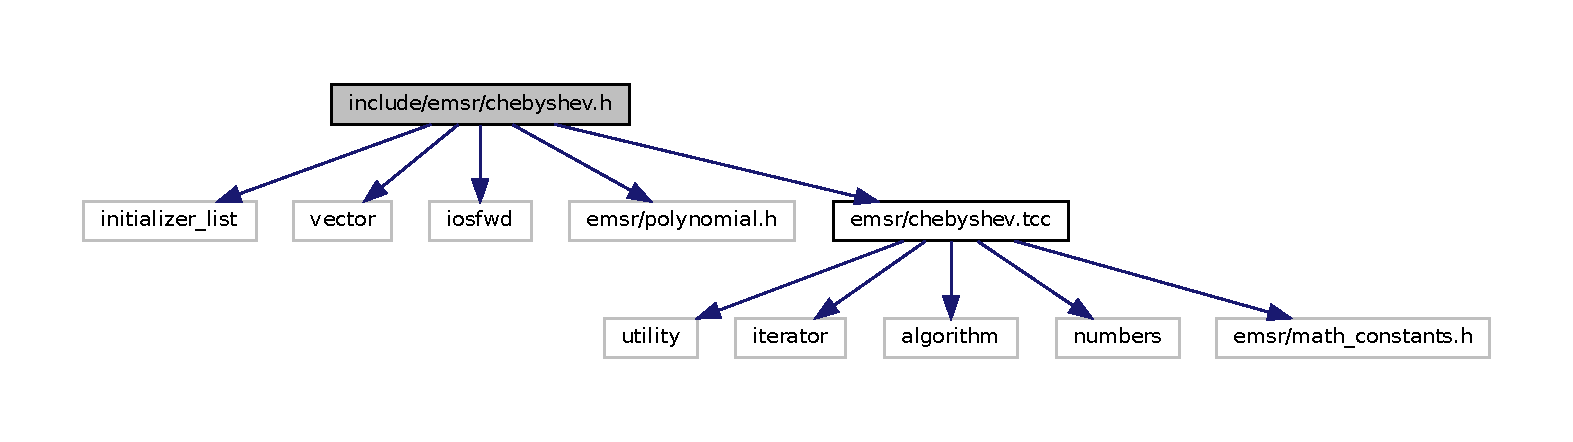
\includegraphics[width=350pt]{chebyshev_8h__incl}
\end{center}
\end{figure}
\subsection*{Classes}
\begin{DoxyCompactItemize}
\item 
class \hyperlink{class____gnu__cxx_1_1__Chebyshev}{\+\_\+\+\_\+gnu\+\_\+cxx\+::\+\_\+\+Chebyshev$<$ \+\_\+\+Tp $>$}
\begin{DoxyCompactList}\small\item\em \hyperlink{class____gnu__cxx_1_1__Chebyshev}{\+\_\+\+Chebyshev} represents a Chebyshev fit of a function. Given a function {\ttfamily func}, the lower limit {\ttfamily a}, the upper limit {\ttfamily b}, and the number of points {\ttfamily n} \hyperlink{class____gnu__cxx_1_1__Chebyshev}{\+\_\+\+Chebyshev} contains the coefficients of a Chebyshev polynomial expansion such that \[ f(x) = k\sum_{0}^{n-1} c_k T_k(x) - c_0/2. \] Use these constructors with moderately large n of 30 or 50. Then truncate the Chebyshev fit to a smaller number of terms to satisfy the accuracy requirements. \end{DoxyCompactList}\end{DoxyCompactItemize}
\subsection*{Namespaces}
\begin{DoxyCompactItemize}
\item 
 \hyperlink{namespace____gnu__cxx}{\+\_\+\+\_\+gnu\+\_\+cxx}
\end{DoxyCompactItemize}


\subsection{Detailed Description}
Interface for C++ Chebyshev methods. 
\hypertarget{chebyshev_8tcc}{}\doxysection{include/emsr/chebyshev.tcc File Reference}
\label{chebyshev_8tcc}\index{include/emsr/chebyshev.tcc@{include/emsr/chebyshev.tcc}}
{\ttfamily \#include $<$utility$>$}\newline
{\ttfamily \#include $<$iterator$>$}\newline
{\ttfamily \#include $<$algorithm$>$}\newline
{\ttfamily \#include $<$numbers$>$}\newline
{\ttfamily \#include $<$emsr/math\+\_\+constants.\+h$>$}\newline
Include dependency graph for chebyshev.\+tcc\+:
\nopagebreak
\begin{figure}[H]
\begin{center}
\leavevmode
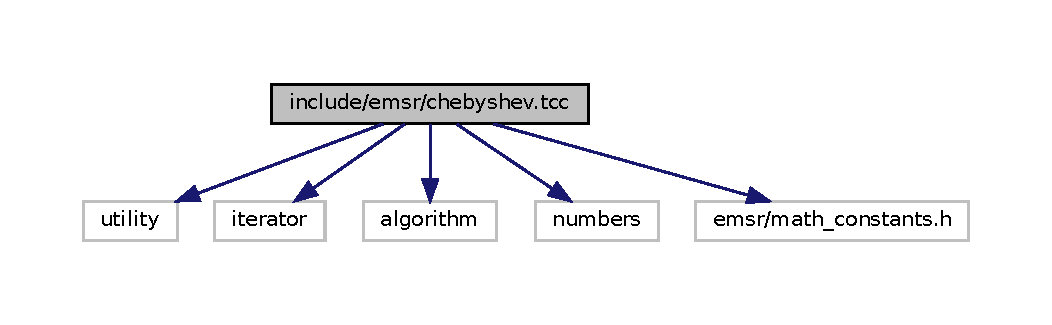
\includegraphics[width=350pt]{chebyshev_8tcc__incl}
\end{center}
\end{figure}
This graph shows which files directly or indirectly include this file\+:
\nopagebreak
\begin{figure}[H]
\begin{center}
\leavevmode
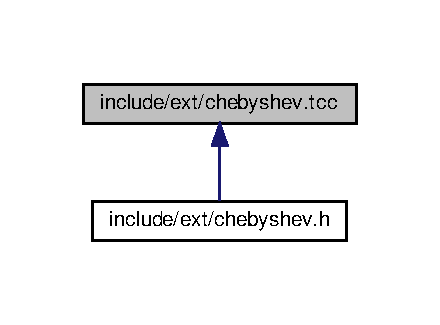
\includegraphics[width=232pt]{chebyshev_8tcc__dep__incl}
\end{center}
\end{figure}
\doxysubsection*{Namespaces}
\begin{DoxyCompactItemize}
\item 
 \mbox{\hyperlink{namespaceemsr}{emsr}}
\end{DoxyCompactItemize}
\doxysubsection*{Macros}
\begin{DoxyCompactItemize}
\item 
\#define \mbox{\hyperlink{chebyshev_8tcc_a0788fa38c6b9d4eb7df643be62450253}{CHEBYSHEV\+\_\+\+TCC}}~1
\end{DoxyCompactItemize}
\doxysubsection*{Functions}
\begin{DoxyCompactItemize}
\item 
{\footnotesize template$<$typename Tp , typename CharT , typename Traits  = std\+::char\+\_\+traits$<$\+Char\+T$>$$>$ }\\std\+::basic\+\_\+ostream$<$ CharT, Traits $>$ \& \mbox{\hyperlink{namespaceemsr_a8a93baa6d2517ab89f043177ff745e9f}{emsr\+::operator$<$$<$}} (std\+::basic\+\_\+ostream$<$ CharT, Traits $>$ \&os, const Chebyshev$<$ Tp $>$ \&cheb)
\item 
{\footnotesize template$<$typename Tp $>$ }\\emsr\+::\+Polynomial$<$ Tp $>$ \mbox{\hyperlink{namespaceemsr_a8a4fd383c8dbd6443f1332ccff289a80}{emsr\+::economize\+\_\+polynomial}} (Tp a, Tp b, const emsr\+::\+Polynomial$<$ Tp $>$ \&poly, Tp eps)
\end{DoxyCompactItemize}


\doxysubsection{Detailed Description}
Implementation for C++ Chebyshev methods. 

\doxysubsection{Macro Definition Documentation}
\mbox{\Hypertarget{chebyshev_8tcc_a0788fa38c6b9d4eb7df643be62450253}\label{chebyshev_8tcc_a0788fa38c6b9d4eb7df643be62450253}} 
\index{chebyshev.tcc@{chebyshev.tcc}!CHEBYSHEV\_TCC@{CHEBYSHEV\_TCC}}
\index{CHEBYSHEV\_TCC@{CHEBYSHEV\_TCC}!chebyshev.tcc@{chebyshev.tcc}}
\doxysubsubsection{\texorpdfstring{CHEBYSHEV\_TCC}{CHEBYSHEV\_TCC}}
{\footnotesize\ttfamily \#define CHEBYSHEV\+\_\+\+TCC~1}


%--- End generated contents ---

% Index
\backmatter
\newpage
\phantomsection
\clearemptydoublepage
\addcontentsline{toc}{chapter}{Index}
\printindex

\end{document}
